% !TeX program = xelatex
% =====================================================================
% 2026 年高教社杯全国大学生数学建模竞赛 C 题
% 微网与外部电网电力调控策略 —— 参赛论文（正文 ≤ 28 页；附录页数不限）
% 版式对照本队提供的三份例文（2024C/2023C/2020C 国奖）与《论文格式规范（2026 修订稿）》
% 编译：xelatex main.tex（连续两次，保证引用与页码正确）
% =====================================================================
\documentclass[10pt,a4paper]{ctexart}

% ---------- 版面（规范：页边距 ≥ 2.5 cm） ----------
\usepackage[top=2.5cm,bottom=2.5cm,left=2.5cm,right=2.5cm]{geometry}

% ---------- 数学与图表 ----------
\usepackage{amsmath,amssymb,bm}
\usepackage{booktabs}
\usepackage{graphicx}
\usepackage{array}
\usepackage{multirow}
\usepackage{caption}
\usepackage{float}
\usepackage{enumitem}
\usepackage{tabularx}
\usepackage{longtable}
\usepackage{tikz}
\usetikzlibrary{arrows.meta,positioning,shapes.geometric}

% ---------- 目录/序号：不用目录；章节用中文序号（例文版式：一、二、三…） ----------
\usepackage{titlesec}
\ctexset{
  section  = {name={,、}, number={\chinese{section}}, format={\bfseries\zihao{4}}, aftername={}, beforeskip={10pt}, afterskip={6pt}},
  subsection = {number={\arabic{section}.\arabic{subsection}}, format={\bfseries\zihao{-4}}, beforeskip={8pt}, afterskip={4pt}},
  subsubsection = {number={\arabic{section}.\arabic{subsection}.\arabic{subsubsection}}, format={\bfseries\zihao{-4}}, beforeskip={6pt}, afterskip={3pt}}
}

% ---------- 公式编号（例文每篇 30~50 个编号公式） ----------
\numberwithin{equation}{section}

% ---------- 页脚中部页码（规范第三条：从摘要页起，阿拉伯数字连续编号） ----------
\usepackage{fancyhdr}
\pagestyle{fancy}
\fancyhf{}
\cfoot{\thepage}
\renewcommand{\headrulewidth}{0pt}
\fancypagestyle{plain}{\fancyhf{}\cfoot{\thepage}\renewcommand{\headrulewidth}{0pt}}

% ---------- 图（150 dpi、宽度 ≤ 0.92 行宽；图注在下） ----------
\graphicspath{{figs/}}
\captionsetup{font=small,labelfont=bf,skip=3pt}
\renewcommand{\figurename}{图}
\renewcommand{\tablename}{表}

% ---------- 附录程序清单（等宽字体用 Consolas，保证希腊字母与符号可正常显示） ----------
\usepackage{listings}
\usepackage{xcolor}
\setmonofont{Consolas}[Scale=0.90]
\lstset{
  basicstyle=\ttfamily\zihao{7},
  breaklines=true, breakatwhitespace=false,
  columns=fullflexible, keepspaces=true,
  showstringspaces=false, frame=single, framesep=3pt,
  numbers=left, numberstyle=\tiny, numbersep=6pt,
  keywordstyle=\color{blue!70!black}, commentstyle=\color{green!40!black},
  stringstyle=\color{red!60!black},
  extendedchars=true, inputencoding=utf8, escapeinside={(*@}{@*)},
  % 不生成“代码目录”条目：本文不设目录，而这些条目会把含长路径的行写进 .aux
  nolol=true,
  % Consolas 缺少若干数学符号；用 literate 在排版时替换为数学字形（不改动任何源程序文件）
  literate={∈}{{$\in$}}1 {⇒}{{$\Rightarrow$}}1 {⁝}{{$\vdots$}}1 {∅}{{$\varnothing$}}1 {≙}{{$\triangleq$}}1 {∪}{{$\cup$}}1 {≪}{{$\ll$}}1 {⌈}{{$\lceil$}}1 {⌉}{{$\rceil$}}1 {⌊}{{$\lfloor$}}1 {⌋}{{$\rfloor$}}1
}
\lstdefinelanguage{PyEx}{language=Python, morekeywords={as,with,None,True,False}}

% ---------- 超链接（不打印彩色边框） ----------
\usepackage[hidelinks,bookmarks=false]{hyperref}

% ---------- 引用编号：排序 + 连续序号压缩为区间（GB/T 7714 写法，如 [28-30]） ----------
% cite 包默认即对同一处 \cite 的多个序号排序并压缩；nocompress / nosort 可关闭。
\usepackage{cite}
% 区间连接符改为中文期刊常用的短横线：如 [28-30]（cite 默认输出 en-dash）
\renewcommand{\citedash}{\hbox{-}\penalty\citepunctpenalty}

% ---------- 浮动体排版：压缩图注间距、允许每页容纳更多图，避免空白页 ----------
\setlength{\textfloatsep}{4.5pt plus 1.5pt minus 1.5pt}
\setlength{\floatsep}{4pt plus 1.5pt minus 1.5pt}
\setlength{\intextsep}{4pt plus 1.5pt minus 1.5pt}
\setcounter{topnumber}{3}
\setcounter{bottomnumber}{2}
\setcounter{totalnumber}{5}
\renewcommand{\topfraction}{0.92}
\renewcommand{\bottomfraction}{0.65}
\renewcommand{\textfraction}{0.06}
\renewcommand{\floatpagefraction}{0.72}
\setlength{\abovedisplayskip}{4.5pt plus 1.5pt minus 1.5pt}
\setlength{\belowdisplayskip}{4.5pt plus 1.5pt minus 1.5pt}
\setlength{\abovedisplayshortskip}{2pt plus 1pt}
\setlength{\belowdisplayshortskip}{2.5pt plus 1pt}
\setlength{\jot}{2pt}
\setlength{\parskip}{0pt plus 0.5pt}
\titlespacing*{\section}{0pt}{7pt}{3.5pt}
\titlespacing*{\subsection}{0pt}{5.5pt}{3pt}
\titlespacing*{\subsubsection}{0pt}{4pt}{2pt}

% ---------- 溢出防护（团队补充，2026-09-12）----------
% 正文含大量 ``13\,758\,182.573724`` 型长数字（\, 处不可断行），行末易产生轻微 Overfull；
% 给行留出弹性伸缩量即可消除，不改变任何内容与数据。
\setlength{\emergencystretch}{3em}
\tolerance=1500
% 表格统一用 tabcolsep 压缩列间距的工具宏（需要时在 table 环境内调用）
\newcommand{\tighttable}{\setlength{\tabcolsep}{4pt}}

% ---------------------------------------------------------------------
\begin{document}

% ============ 第 1 页：摘要专用页（电子版首页） ============
\begin{center}
  {\zihao{3}\bfseries 基于逐时段线性规划与滚动调整的\linebreak 微网购电—储能调度策略}
\end{center}
\vspace{2pt}

\section*{摘\quad 要}
微网通过在外部电网电价低谷或分布式光伏盈余时段为储能充电、在电价高峰时段放电，可在满足小区负载的前提下降低购电费用。本文建立\textbf{统一的逐时段确定性线性规划框架}，把时间分辨率、信息结构、结算制度与电价情景四个维度分别参数化，依次求解四个问题，交付 \texttt{result1.xlsx}、\texttt{result2.xlsx}、\texttt{result3.xlsx}、\texttt{result4-2.xlsx}、\texttt{result4-3.xlsx} 五个结果文件。

\textbf{模型与思路。} 以 10 分钟为决策时段，决策变量为计划购电量、调整购电量、紧急购电量、充放电量与弃光量，状态量为储电量。功率平衡取等式，储能动态计入 90\% 双向效率（往返 81\%），容量与功率约束按题面附录。目标为购电费用最小且\textbf{不乘时段长}。本文给出互补性引理：往返效率小于 1 且电价为正时，“同时充放电”被“少充少放”严格支配，故线性松弛无损、无需二元变量；鉴于最优调度面可能不唯一，全部模型统一按固定规则选取输出的解。

\textbf{主要结果。} 问题一在附件 1 的代表性单日上得最优全天购电费 $35126.948589$ 元、购电量 $59482.698998$ kWh，呈典型的分时电价套利形态，最便宜的 20\% 电价时段承担 55.4\% 的充电量，日周期精确闭合、全日无弃光。问题二把模型滚动到全年 365 天（52\,560 时段），得全期购电费 $13\,758\,182.573724$ 元、交付期（2 月 1 日—12 月 31 日，334 天）$12\,233\,050.830708$ 元，并证明在“完全信息 + 无购电上限”下紧急购电恒为零。问题三引入附件 3 整点光伏预报的降尺度与 6:00、12:00、18:00 三个调整时刻及 $0.5\times/1.5\times$ 双向分段结算，交付期费用升至 $14\,540\,616.335652$ 元，比问题二高 $2\,307\,565.50$ 元（$+18.863\%$），该差额即预报误差的代价。问题四在附件 4 的实时波动电价下重算问题二与问题三，两条链的交付期费用分别为 $13\,006\,411.041148$ 元与 $15\,289\,050.714738$ 元；两链差额 $2\,282\,639.673590$ 元可\textbf{完全归因}为计划量差异 $100\,230.446225$ 元、偏差结算 $522\,512.788776$ 元与紧急购电 $1\,659\,896.438588$ 元三项。按“0:00 时当日电价未知”的处理方式，决策层使用由历史价格构造的预测价、结算一律用实际价，价格预报误差的代价为 $520\,790.839035$ 元与 $258\,485.465704$ 元。

\textbf{验证与稳健性。} 四问均通过五项独立检验：结果完整性、144 时段独立回代、量纲与逐层目标复算、解析界与常识检验、跨问题一致性五级验收，等式残差不超过 $4.6\times10^{-12}$，交付工作簿逐格复算一致。问题一判“稳定”，问题二判“脆弱（需缩小适用范围）”，问题三与链 \emph{4-3} 判“条件稳定”，链 \emph{4-2} 判“稳定”；全部未通过的检验与反例均如实列出，未通过调参或放宽阈值使其“通过”。

\textbf{创新点。} 以四个维度上的参数化统一四问并形成可复用模板；用互补性引理把“是否需要二元变量”从工程判断变为数学结论；把不确定性代价拆成可计价的分项；用退化情景复现构造实现正确性基准（六项指标逐位复现，相对差不超过 $4.86\times10^{-13}$）；用只改“看多远”的滚动时域对照回答结构性问题；并对“是否需要更多预报、是否需要随机优化”给出三层递进的定量回答。不足在于文献证据仅达摘要/元数据级、未显式强制充放电互补、若干物理简化，以及全部结果基于确定性点预测，已在正文逐条说明。


\vspace{4pt}
\noindent\textbf{关键词}：微网调度；储能运行优化；线性规划；分时电价套利；偏差分段结算；滚动时域优化；价格预报误差

\newpage

% ============ 正文 ============
\section{问题重述}

\subsection{问题背景}

微网是为解决光伏发电等分布式能源的本地消纳、减少并网问题而发展起来的小型发用电系统。出于经济方面的考虑，非孤岛式微网可在外部电网（以下简称外网）电价较低或分布式能源有剩余电量的时段为储能设备充电，并在外网电价较高的时段释放电能；其调控目标是在利用小区负载、光伏发电量与储能当前储电量等数据的前提下，尽可能精准地给出微网的购电量与储能设备的充放电量，使微网提供的电力既满足小区负载、又尽可能节省购电费用。

题面附录给出储能设备参数：最大容量 12000 kWh，最大充放电功率 5000 kW，2025 年 1 月 1 日 0:00 的电量为 6000 kWh，运行过程中电量须保持在 $1200$--$10800$ kWh 之间，充放电效率为 90\%。

\subsection{问题提出}

\textbf{问题一}要求建立每天 0:00 制定当天计划购电策略的数学模型：电价与小区负载逐日相同、光伏发电功率有一天预测数据；微网提供的电能不得低于小区负载；储能设备在 0:00 与 24:00 的储电量相同；目标为全天购电费用最小。需基于附件 1 给出计划购电策略与充放电安排，保存为 \texttt{result1.xlsx}。

\textbf{问题二}把决策期扩展到全年：电价仍逐日相同，而负载与光伏逐日变化；若微网提供的电能低于负载，需向外网紧急购电，电价为交易时刻电价的 5 倍；除紧急购电外，其余购电费用按计划购电量计算。需基于附件 1 电价与附件 2 实际负载、实际光伏，在每天 0:00 制定当天计划，给出四个指定日期（2025 年 3 月 20 日、6 月 21 日、9 月 23 日、12 月 21 日）的结果与紧急购电结果，保存为 \texttt{result2.xlsx}。

\textbf{问题三}引入光伏功率的滚动预报：每天 0:00、6:00、12:00、18:00 可获得未来 24 小时整点预报。可依据 0:00 预报制定当天计划，也可依据其他时刻预报调整购电策略；计划购电量高于调整购电量时，违约电价为交易时刻电价的 50\%；调整购电量高于计划购电量时，超出部分电价为交易时刻电价的 1.5 倍；总费用包括计划购电费用、紧急购电费用与调整购电量的相关费用。需基于附件 1、2、3 建立模型、给出四个指定日期的结果并保存为 \texttt{result3.xlsx}，并分析是否需要引入其他时刻的预报来制定调整策略。

\textbf{问题四}指出外网电价本身也是实时波动的，要求在附件 4 的实时波动电价情景下，利用附件 2 的负载与光伏、附件 3 的光伏预报，\emph{重新计算问题二与问题三}，并分别保存为 \texttt{result4-2.xlsx}（对应问题二）与 \texttt{result4-3.xlsx}（对应问题三）。

由题面可见，问题四在数学上等价于\textbf{两道题}。二者共用附件 4 电价，但决策结构与结算方式不同：重算问题二只有每天一次的日计划与 5 倍价紧急购电，重算问题三则另有三个调整时刻与 $0.5\times/1.5\times$ 分段结算。因此本文自始至终按两条独立的结果链组织计算与验收，分别记为链 \emph{4-2} 与链 \emph{4-3}；两链共用同一价格预测器与同一结算方式（结算一律用实际电价）。

\section{问题分析}

\subsection{总体分析}

四个问题的物理系统完全相同：一张光储微网与一个外部电网相连，储能设备的容量、功率、效率与运行区间由题面给定，光伏先供负载、盈余充入储能、不足由外网补足。因此四问的差异不在物理规律，而在\textbf{决策者知道什么、什么时候决定、按什么规则结算}三件事上。据此本文把四个问题统一抽象为四个维度上的参数化：

\begin{enumerate}[leftmargin=2em,itemsep=1pt]
  \item \textbf{时间维度}（决策时刻集合）：问题一、二每天只有一个决策时刻；问题三与链 \emph{4-3} 有 0:00、6:00、12:00、18:00 四个决策时刻，后续时刻可修改先前的决定。
  \item \textbf{信息维度}（各层信息集）：问题一、二的计划层被视为完全信息；问题三的计划层只知 0:00 发布的整点预报，调整层另可见当天已实现时段；链 \emph{4-2}、\emph{4-3} 在 0:00 时对当日实时电价一无所知，只能用历史价格。
  \item \textbf{结算维度}（超额与不足如何计价）：问题一、二只有“按计划量计费”与“紧急购电按 5 倍价”两条规则；问题三与链 \emph{4-3} 另有 $0.5\times/1.5\times$ 双向分段结算。
  \item \textbf{价格情景维度}：电价是逐日重复的单日曲线（附件 1），还是逐日波动且当日不可预知的实际序列（附件 4）。
\end{enumerate}

这一抽象带来两个好处：四个问题共用一套平衡方程、储能动态、容量与功率约束和目标函数，模型规模与正确性可用同一套方法核验；同时“难点”被定位到具体维度上，“是否需要更多时刻的预报”“要不要做随机优化”“日边界为什么总贴储电量下限”这类问题都有了明确的讨论对象。技术路线如图~\ref{fig:roadmap}。

\begin{figure}[htbp]
\centering
\begin{tikzpicture}[font=\footnotesize,
  box/.style={draw,rounded corners=2pt,align=center,inner sep=3pt,minimum height=6.5mm},
  core/.style={box,fill=black!7,thick},
  dim/.style={box,fill=black!2,dashed},
  ar/.style={->,>=stealth,thick}]
\node[dim] (d1) at (0,2.0) {时间维度\\决策时刻集合};
\node[dim] (d2) at (2.9,2.0) {信息维度\\各层信息集};
\node[dim] (d3) at (5.8,2.0) {结算维度\\超额/不足计价};
\node[dim] (d4) at (8.7,2.0) {价格情景\\附件 1 / 附件 4};
\node[core] (lp) at (4.35,0.6) {统一逐时段确定性线性规划内核\\平衡方程 $\cdot$ 储能动态 $\cdot$ 容量与功率约束 $\cdot$ 费用目标};
\node[box] (p1) at (0,3.4) {问题一\\单日计划};
\node[box] (p2) at (2.9,3.4) {问题二\\全年计划 + 紧急购电};
\node[box] (p3) at (5.8,3.4) {问题三\\计划 + 调整 + 分段结算};
\node[box] (p4) at (8.7,3.4) {问题四\\两条链并行};
\draw[ar] (d1) -- (lp); \draw[ar] (d2) -- (lp); \draw[ar] (d3) -- (lp); \draw[ar] (d4) -- (lp);
\draw[ar] (lp) -- (p1); \draw[ar] (lp) -- (p2); \draw[ar] (lp) -- (p3); \draw[ar] (lp) -- (p4);
\end{tikzpicture}
\caption{技术路线：在四个维度上参数化的统一线性规划内核}
\label{fig:roadmap}
\end{figure}

\subsection{各问题的关键难点}

\textbf{问题一}的输入（附件 1 的电价、负载与光伏预测）均视为确定值，约束中真正起作用的是储能：容量上下限、两侧功率上限、往返效率 81\%，以及“0:00 与 24:00 储电量相等”的日周期条件。经济上这是典型的跨时段套利：储能把电能从低价时段搬到高价时段，搬运损耗表现为往返效率小于 1。需要论证的是两件事：是否需要二元变量强制“不同时充放电”；光伏盈余超过储能吸收能力时功率平衡如何闭合。

\textbf{问题二}需处理三点新结构。其一，日周期约束被\textbf{跨日状态连续性}取代——题面只在问题一要求端点储量相同，把该约束逐日施加会人为割裂跨日搬运电能的可能性，本文用逐日解耦的对照量化这一差别。其二，\textbf{终端条件必须显式声明}：题面未规定决策期末储电量，若允许自由终止，模型会把期末库存“变卖”以压低账面费用，本文保留终端自由但把该效应单独计价。其三，\textbf{紧急购电在完全信息下不会被激活}：既然 0:00 已知当天实际负载与光伏、且购电无功率上限，任何“先欠着、事后按 5 倍价补”都可事先改为按正常价买入同样电量而严格更省。该结论是模型内的推论而非实测断言，也不意味着机制可删——一旦引入购电上限，紧急购电立即被激活。

\textbf{问题三}的关键变化是\textbf{信息结构}：附件 3 只给整点预报，而决策与结算以 10 分钟为粒度。由此产生两个必须处理的环节：\emph{降尺度}（本文取整点锚定线性插值，该口径不保证块内能量守恒，其影响可能大于调整机制本身，故作为独立消融项量化）与\emph{非预期性}（0:00 计划只能用 0:00 预报，调整只能用该时刻已发布预报与已实现状态，不得使用未来实际值）。因此模型被组织为三层顺序向前递推，而非能“看到未来”的联合优化。此外，由于决策层用预报、结算层用实际光伏，预报误差必然造成缺口；调整降低了紧急购电却引入偏差违约金，其净效果只能用同一口径下的费用分解回答。

\textbf{问题四}的实质是\textbf{价格可观测性}的改变。“实时”意味着 0:00 制定当天计划时当天 144 个电价点尚未发生；若直接把附件 4 当作已知输入，就等于假设电价可完全预知。本文明确采用“决策层用历史价格构造的预测价、结算层一律用实际价”的口径，并把二者差额定义为“价格预报误差的代价”单独报告。由此两条链的性质不同：链 \emph{4-2} 中价格不确定性只改变费用、不产生能量缺口；链 \emph{4-3} 中缺口来自光伏预报误差，价格不确定性则同时影响计划层、调整层的决策与最终账单。两链费用差额可完全分解为计划口径差、偏差结算与紧急购电三项。同时，两链都采用“当天决策、终端自由”的组织方式，日边界储电量会贴住下限——这究竟是普遍性质还是特定结构的产物，需要改变前瞻深度的对照实验来回答。

\section{模型假设}

结合题面条件与数据的实际结构，本文作如下假设。凡属题面未规定而由本文约定的做法，均在条目中直接说明，不以隐含默认的方式使用。

\begin{enumerate}[leftmargin=2.4em,itemsep=2pt]
  \item \textbf{时间离散与对齐}：电价、负载与光伏功率均以 10 分钟为时段、每日 144 段；附件时间戳为所属时段的\emph{左端点}，第 $i$ 个数据点代表区间 $[10i,10i+10)$ 分钟，与结果模板的 144 个时段按位置一一对应。据此计划窗为 0:10 至 24:10，模板标称的“0:00--4:00”等标签对应物理区间整体前移 10 分钟，属模板固有相位，全文表格与图注均按此约定统一。
  \item \textbf{时段内恒定}：每个时段内电价与功率视为常数，时段电量等于功率乘以 $\Delta t=1/6$ h；反之，以电量表示的决策变量本身已含时间因子，费用表达式中不再乘以 $\Delta t$。
  \item \textbf{储能模型}：储能按常效率模型描述，充、放电各按 90\% 计（往返效率 81\%），静置时不发生自放电；容量运行区间为 $[1200,10800]$ kWh，初始储电量为 6000 kWh。
  \item \textbf{功率上限的作用位置}：题面“最大充放电功率 5000 kW”同时作用于并网点侧与电池侧、取更严者，故充电量上界为 $5000\Delta t=833.3333$ kWh、放电量上界为 $5000\Delta t\,\eta=750.0000$ kWh。该项为题面参数的解释约定，本文不将其表述为文献结论。
  \item \textbf{弃光变量保留}：光伏盈余中未被负载与储能消纳的部分记为弃光量 $s$，其目标系数为零（无上网售电收益），但变量必须保留，以便在盈余超出储能吸收能力的时段闭合功率平衡。
  \item \textbf{购电无功率上限、无售电收益}：外网购电量非负且不设上界；光伏余电不上网，储能也不向电网售电。当分析中引入购电上限或售电价格时，均视为独立的结构性对照情景单独报告。
  \item \textbf{费用范围}：目标只计购电费用，不引入折旧、循环寿命或退化成本（题面未给系数，无法标定）。紧急购电按交易时刻电价的 5 倍计价；问题三与链 \emph{4-3} 中，计划高于最终的部分按 0.5 倍价、最终高于计划的部分按 1.5 倍价计价，两段均为成本项而非退款，且以当天 0:00 计划为唯一基准、单次结算、不回溯。
  \item \textbf{信息非预期性}：任一决策时刻只能使用该时刻已发布或已实现的数据。问题三与链 \emph{4-3} 中，0:00 计划层只用 0:00 预报，6:00、12:00、18:00 调整层只用该时刻已发布预报加已实现状态；实际光伏只进入事后结算层，不影响任何决策量与储能轨迹。
  \item \textbf{价格可观测性}：在附件 4 的波动电价情景下，0:00 制定当天计划时当天实时电价尚未发生、不可观测，决策层只能使用由历史价格构造的预测价，而费用结算一律使用实际电价；由此产生的决策—结算差异单独量化为“价格预报误差的代价”。
  \item \textbf{供电可靠性由等式平衡保证}：每个时段采用等式功率平衡并显式包含紧急购电与弃光变量，由此“微网提供的电能不低于小区负载”自动成立、充电不挤占负载；模型不进一步建模切负荷。
  \item \textbf{数据可用性与预报边界}：附件 2--4 在 2025 全年无缺日、无重复，附件 3 的日期列存在前向填充结构，读取时按前向填充还原；题面只提供未来 24 小时的整点光伏预报，本文不假设可获得更长时间跨度或更高时间分辨率的预报。
\end{enumerate}

此外，由于最优调度面可能不唯一（储电量上下限两端均可能活跃），本文统一约定一条\textbf{解的选择规则}：所有模型、所有层先在主目标最优面上取解，再在其中最小化储能吞吐量（字典序规则）。验收一律以约束残差、结构恒等式、目标值与交付表格为准，不比对逐点解的唯一性。

\section{符号说明}

四个问题共用同一套符号。电量类变量以 kWh 为单位、本身已含时间因子；功率类输入以 kW 为单位；费用类量以元为单位。

\begin{center}
\small
\begin{tabular}{clc}
\toprule
符号 & 含义 & 单位 \\
\midrule
$t,\ \tau$ & 时段索引，每日 $t=1,\dots,144$；全年 $\tau=1,\dots,52560$ & --- \\
$d,\ i$ & 日期索引（全年 365 天）；日内 10 分钟时段索引 $i=1,\dots,144$ & --- \\
$m$ & 决策时刻，$m\in\{0,6,12,18\}$ & h \\
$\Delta t$ & 时段长度，$\Delta t=1/6$ & h \\
$L_t$ & 小区负载功率 & kW \\
$PV_t$ & 光伏发电功率；$PV^{fc}_t$ 为预报值，$PV^{act}_t$ 为实际值 & kW \\
$p_t$ & 电价（问题一至三取自附件 1，逐日重复） & 元/kWh \\
$p^{act}_{d,i}$ & 附件 4 的实际波动电价 & 元/kWh \\
$\hat p^{(m)}_{d,i}$ & 决策时刻 $m$ 信息集下的预测电价；$\kappa_m$ 为调整层的水平校正因子 & 元/kWh \\
$b_t$ & 计划购电量（0:00 制定） & kWh \\
$q_t$ & 调整后的最终购电量（替代量口径） & kWh \\
$q^{em}_t$ & 紧急购电量（缺口部分） & kWh \\
$c_t,\ q^{dis}_t$ & 储能充电量、放电量 & kWh \\
$s_t$ & 弃光量（光伏盈余中未被消纳的部分） & kWh \\
$E_t$ & 时段末储电量（状态变量） & kWh \\
$\eta$ & 充放电效率，$\eta_{ch}=\eta_{dis}=0.9$ & --- \\
$E_{\min},E_{\max}$ & 储电量运行区间，$1200$ 与 $10800$ & kWh \\
$E_{\text{init}}$ & 初始储电量（2025-01-01 0:00），6000 & kWh \\
$P_{\max}$ & 最大充放电功率，5000 & kW \\
$\alpha_{em}$ & 紧急购电电价倍数，$\alpha_{em}=5$ & --- \\
$\beta_{def},\beta_{over}$ & 偏差结算倍数，$\beta_{def}=0.5$，$\beta_{over}=1.5$ & --- \\
$C_{\text{plan}},C_{\text{adj}},C_{\text{em}}$ & 计划购电费、偏差结算费、紧急购电费 & 元 \\
$C_{\text{total}}$ & 总费用 $C_{\text{plan}}+C_{\text{adj}}+C_{\text{em}}$ & 元 \\
$C^{fc}$ & 同一组决策按决策层信念价计得的费用 & 元 \\
$N$ & 净负荷电量 $\sum_t(L_t-PV_t)\Delta t$ & kWh \\
$D_{\text{full}},D_{\text{req}}$ & 全年 365 天；交付期 2025-02-01 至 12-31 共 334 天 & --- \\
$T$ & 决策期时段总数（问题二为 52\,560） & --- \\
\bottomrule
\end{tabular}
\end{center}

需要特别说明两处容易混用、一旦混用就无法比对的量：其一，$b$ 与 $q$ 是两个不同的量，$b$ 是 0:00 制定的计划购电量，$q$ 是该时段\emph{最终}的购电量（替代量口径而非增量），问题三与链 \emph{4-3} 的交付表报的是 $q$；其二，“全期”指 365 天，“交付期”指 2025 年 2 月 1 日之后的 334 天，1 月作为储能预热期不计入交付——全文出现的每一个费用数字都标注其所属口径。


\section{模型的建立与求解}
\subsection{数据预处理与特征分析}

\subsubsection{输入数据与口径}

四个问题的输入来自附件 1--4，其用途与读取口径如表~\ref{tab:data}。需要说明的是：附件 1 中的负载与光伏预测列只服务于问题一的“单日代表”语义，附件 3 的光伏预报只服务于问题三与链 \emph{4-3}，附件 4 的电价只服务于问题四。各问题的输入边界在建模时即已固定，不做跨问题借用，以保证四个问题之间互不“串答案”。

\begin{table}[htbp]
\centering
\small
\caption{输入数据及其在各问题中的用途}
\label{tab:data}
\begin{tabular}{p{1.8cm}p{3.4cm}p{7.0cm}}
\toprule
数据 & 结构 & 用途与读取口径 \\
\midrule
附件 1 & 145 行 $\times$ 4 列，10 分钟粒度单日 & 问题一至三的电价（逐日重复 365 次）；问题一的负载与光伏预测。电价取值于 $[0.3713,1.3952]$ 元/kWh，144 点之和为 110.3324 元/kWh \\
附件 2 & 365 行 $\times$ 144 列，实际值 & 问题二至四的负载与光伏实际功率。负载取值于 $[1995.7176,7978.8849]$ kW，光伏取值于 $[0,10216.20]$ kW \\
附件 3 & 365 天 $\times$ 4 个发布时刻 $\times$ 24 小时 & 问题三与链 \emph{4-3} 的整点光伏预报，需降尺度到 10 分钟 \\
附件 4 & 366 行 $\times$ 145 列，实时电价 & 问题四唯一的价格来源。取值于 $[0.0076,1.7936]$ 元/kWh，全期均值 0.7661976 元/kWh \\
模板文件 & 附件 5 的 5 个结果文件 & 决定表格结构与填报口径；模板中的数值不作为任何结论依据 \\
\bottomrule
\end{tabular}
\end{table}

附件 4 有三个值得注意的统计事实。第一，电价存在极端低值：全期最小值为 0.0076 元/kWh，低于 0.10 元/kWh 的时段仅 28 个，因此以最小电价构造的费用下界极为宽松（不足实际费用的 1.2\%），量级自检必须改用构造性上界。第二，深谷时段的 5 倍紧急购电价仅为 0.038 元/kWh，讨论惩罚机制时不能用全期均价外推。第三，附件 4 的\textbf{日内形状与附件 1 的电价曲线高度一致}：同时段跨日均值曲线与附件 1 曲线的相关系数为 0.9999999956（四位小数即为 1.0000）且极值位置相同，差异体现为日间水平漂移（日均价在 0.5378 至 0.9290 元/kWh 之间）叠加逐点扰动。这既解释了附件 1 电价能被逐日重复使用的原因，也说明在波动电价情景下采用“水平 $\times$ 时段”的双因子预测器有数据依据。

数据覆盖 2025 年 1 月 1 日至 12 月 31 日共 365 天、无缺日无重复；按结果文件要求，交付期为 2025 年 2 月 1 日至 12 月 31 日共 334 天，1 月作为储能预热期参与滚动递推但不计入交付。全部问题均自 2025 年 1 月 1 日 0:00 的 6000 kWh 起算，日间通过储电量连续性衔接，不施加逐日周期约束。

\subsubsection{负载与光伏的结构特征}

全年 52\,560 个时段中，出现光伏功率大于负载功率（即存在盈余）的时段有 10\,130 个，占 19.3\%。这类时段是储能充电的天然窗口，也是弃光可能发生的时段。交付期净负荷电量为 17\,939\,189.494967 kWh，该数值只与附件 2 有关，因此在问题二、问题三、链 \emph{4-2} 与链 \emph{4-3} 中\textbf{逐位相同}——它构成一个有用的交叉校验量：若某个模型算出的净负荷与此不符，说明取数或时间对齐出错。

由图~\ref{fig:input} 可见，负载在午间与傍晚出现双峰，光伏在正午达到最大，于是净负荷在正午被光伏压得很低、在傍晚急剧抬升。这意味着低价充电窗口集中在凌晨与正午、高价放电窗口集中在傍晚与夜间，正是分时电价套利的典型场景；而充放电之间的能量搬运要付出 19\% 的往返损耗，因此只有当价差足以覆盖损耗时套利才发生。

\begin{figure}[htbp]
\centering
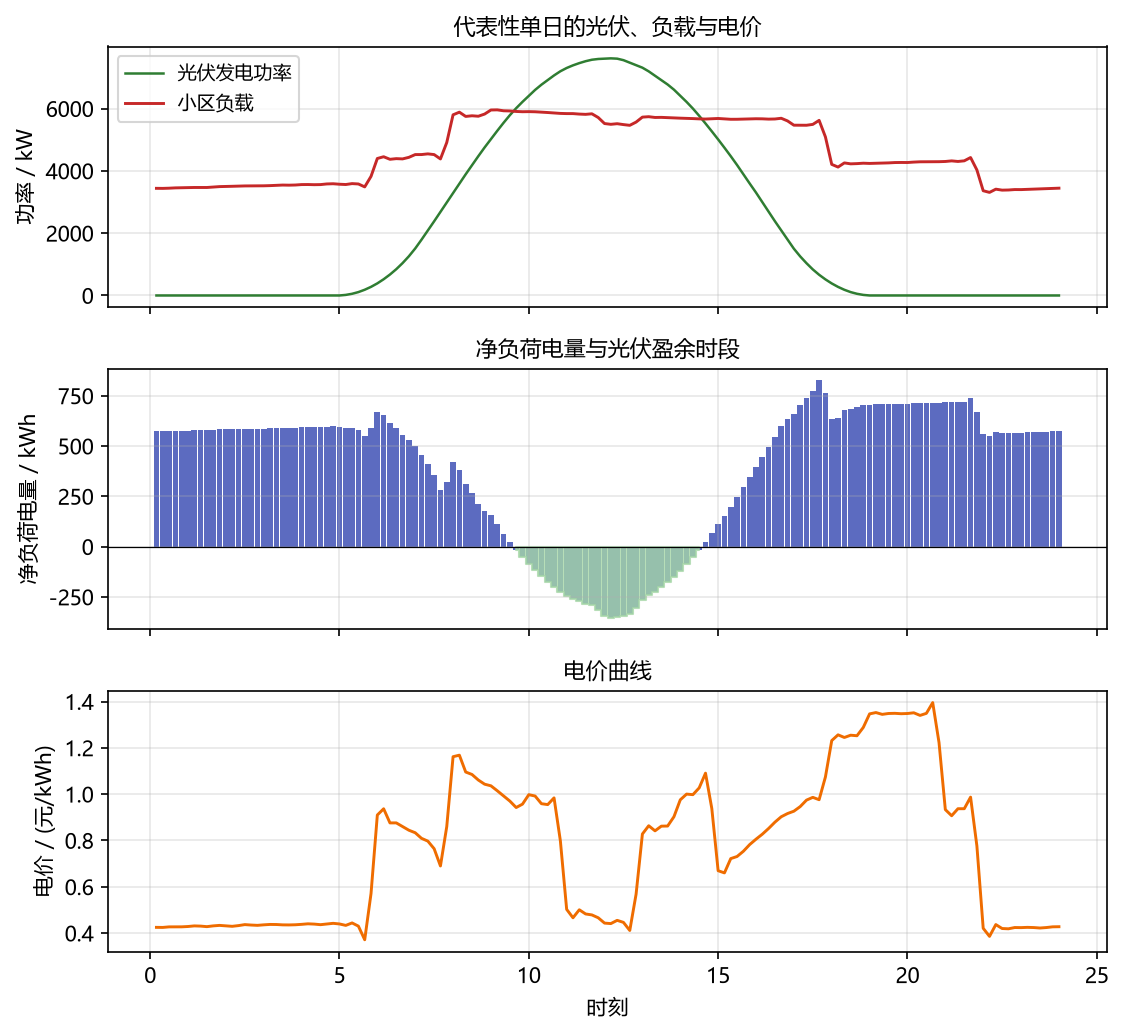
\includegraphics[width=0.80\textwidth]{fig01_inputs.png}
\caption{附件 1 代表性单日的电价、小区负载与光伏预测功率，以及净负荷电量}
\label{fig:input}
\end{figure}

\subsubsection{异常与边界检查}

对全部输入做了四项检查：其一，缺失与重复检查——附件 2--4 无缺日无重复，附件 3 的日期列按前向填充还原为 365 天 $\times$ 4 个发布时刻；其二，量纲检查——功率乘以 $\Delta t$ 得电量，费用等于电价与电量之积且不乘 $\Delta t$；其三，时序一致性检查——附件 1 与附件 2 的 144 点采用同一左端点口径，若误用右端点会使全部时段整体错位 10 分钟；其四，净负荷一致性检查——四问共用同一净负荷数值。上述检查在每次计算后都以只读方式重新执行，检查脚本与计算脚本相互独立。

\subsection{统一优化框架}

\subsubsection{模型结构}

四个问题共用同一组决策变量：计划购电量 $b$、最终购电量 $q$、紧急购电量 $q^{em}$、充电量 $c$、放电量 $q^{dis}$ 与弃光量 $s$，并以时段末储电量 $E$ 为状态变量。以问题二为例，全年模型为

\begin{equation}
\begin{aligned}
\min_{b,\,q^{em},\,c,\,q^{dis},\,s,\,E}\quad
& C_{\text{total}}=\sum_{\tau=1}^{T}\Bigl(p_{\tau}b_{\tau}+\alpha_{em}p_{\tau}q^{em}_{\tau}\Bigr),
\quad \alpha_{em}=5,\quad T=52560
\end{aligned}
\end{equation}

\begin{equation}
\text{s.t.}\quad
b_{\tau}+q^{em}_{\tau}+PV_{\tau}\Delta t+q^{dis}_{\tau}=L_{\tau}\Delta t+c_{\tau}+s_{\tau},
\qquad 0\le s_{\tau}\le PV_{\tau}\Delta t
\end{equation}

\begin{equation}
0\le c_{\tau}\le 5000\Delta t=833.3333,\qquad
0\le q^{dis}_{\tau}\le 5000\Delta t\,\eta=750.0000
\end{equation}

\begin{equation}
E_{\tau}=E_{\tau-1}+\eta c_{\tau}-\frac{q^{dis}_{\tau}}{\eta},\qquad
\eta=0.9,\qquad 1200\le E_{\tau}\le 10800,\qquad E_{0}=6000
\end{equation}

\begin{equation}
b_{\tau}\ge0,\quad q^{em}_{\tau}\ge0,\quad c_{\tau}\ge0,\quad q^{dis}_{\tau}\ge0,\quad s_{\tau}\ge0
\end{equation}

式 (2) 的等式平衡使“供电不低于负载”自动成立，同时充电不与负载竞争；这一形式化与微网并网储能系统的逐时段成本最小建模传统一致\cite{ref-csee-2023-mg-ems-review,ref-moradi-2018-standalone,ref-alguhi-2025-bess-operation,ref-valibeygi-2020-battery-dispatch-soc}。模型规模为变量 $6T=315\,360$ 个、等式约束 $2T=105\,120$ 条、非零元 $9T-1=473\,039$ 个、整数变量 0 个；矩阵高度稀疏（非零元占比约 $1.4\times10^{-5}$），实现时采用稀疏存储，稠密存储需约 265 GB 内存并不可行。

\subsubsection{三处需要论证的建模要点}

\textbf{其一，是否需要二元变量强制“不同时充放电”。} 直观上储能不应在同一时段既充电又放电。本文不引入二元变量，而用如下引理保证线性松弛无损。

\begin{quote}
\textbf{引理 1（互补性）} 若 $\eta^2<1$ 且电价 $p_{\tau}>0$，则任一同时充放电的解都不是严格最优解；模型存在满足 $c_{\tau}q^{dis}_{\tau}=0$ 的最优解。

\textbf{证明} 设某时段 $c_{\tau}>0$、$q^{dis}_{\tau}>0$，令 $\varepsilon=\min(c_{\tau},q^{dis}_{\tau})>0$，把二者同时减去 $\varepsilon$：储电量净变化为 $-\eta\varepsilon+\varepsilon/\eta>0$（因 $\eta^2<1$），状态反而上升。因此可再把充电量减去 $\eta^2\varepsilon$，即取 $c'_{\tau}=c_{\tau}-\varepsilon$、$q^{dis\prime}_{\tau}=q^{dis}_{\tau}-\eta^2\varepsilon$，此时状态净变化恰为 $-\eta\varepsilon+\eta^2\varepsilon/\eta=0$，状态轨迹完全不变。该修改使购电量减少 $\varepsilon(1-\eta^2)>0$，费用严格下降，与最优性矛盾。故存在最优解满足互补性。$\square$
\end{quote}

引理 1 说明“不需要二元变量”是精确性质而非近似；其代价是最优面可能不唯一，故本文统一采用字典序规则选取提交解。同一现象在电池调度文献中亦被讨论：当往返效率小于 1 时线性松弛的互补性可以自发满足，而强制互补会带来数值与规模上的额外代价\cite{ref-wang-2024-complementarity,ref-nazir-2023-realizable-dispatch}。

\textbf{其二，光伏盈余如何闭合。} 附件 1 的光伏峰值 7612.32 kW 高于负载峰值 5958.97 kW，附件 2 中也有相当比例的时段光伏超过负载。若不加弃光变量而要求等式平衡，模型在这些时段将不可行；若改为不等式（净供给不低于负载），余电可以凭空消失，会低估可行域并扭曲费用。本文采用等式平衡加显式弃光变量（$s\in[0,PV\Delta t]$、目标系数为零）的做法：盈余只能被储能吸收或以 $s$ 弃掉，既不凭空消失也不上网售电。光伏限出力在含储能的经济调度中通常以同样的方式显式建模\cite{ref-grimaldi-2025-arbitrage-curtail,ref-qing-2025-pv-curtailment}。

\textbf{其三，终端条件。} 题面未规定决策期末的储电量，本文保留终端自由，只要求其落在运行区间内。由于期末库存具有经济价值，终端自由会使模型在末期“放空”储能，这一效应在结果中被显式量化（问题二为 $+2217.08$ 元），以免与价格套利混淆。

\subsubsection{结构恒等式}

对任意可行解，把储能状态转移式在决策期上求和可得两条与目标函数无关的恒等式，它们是比目标值更严格的正确性检验：

\begin{equation}
\sum_{\tau}q^{dis}_{\tau}=\eta^2\sum_{\tau}c_{\tau}-\eta\bigl(E_{T}-E_{0}\bigr)
\end{equation}

\begin{equation}
\sum_{\tau}b_{\tau}=N+\sum_{\tau}s_{\tau}+\bigl(1-\eta^2\bigr)\sum_{\tau}c_{\tau}
+\eta\bigl(E_{T}-E_{0}\bigr)-\sum_{\tau}q^{em}_{\tau},
\qquad N=\sum_{\tau}\bigl(L_{\tau}-PV_{\tau}\bigr)\Delta t
\end{equation}

式 (8) 的含义是：全年购电量等于净负荷加上弃光、加上储能循环损耗，再扣除期末放空的库存。以问题二为例，$\eta(E_T-E_0)=0.9\times(1200-6000)=-4320$ kWh，即期末放空等价于少购 4320 kWh；这条账在四个问题中都被独立复核，残差为零。

\subsubsection{四个维度上的参数化}

四个问题不需要分别推导模型，只需在表~\ref{tab:param} 的四个维度上取不同取值。

\begin{table}[htbp]
\centering
\footnotesize
\caption{四个问题在统一框架下的参数化}
\label{tab:param}
\begin{tabular}{p{1.4cm}p{2.4cm}p{3.4cm}p{3.6cm}p{2.6cm}}
\toprule
 & 时间维度 & 信息维度 & 结算维度 & 价格情景 \\
\midrule
问题一 & 单日 144 段 & 完全信息 & 按计划量计费 & 单日曲线（附件 1） \\
问题二 & 全年 52\,560 段 & 完全信息 & 计划量计费 + 5 倍紧急购电 & 逐日重复（附件 1） \\
问题三 & 全年，四个决策时刻 & 预报驱动（附件 3） & 上述 + 0.5/1.5 倍双向分段 & 逐日重复（附件 1） \\
链 \emph{4-2} & 全年，每日 0:00 & 负载/光伏完全信息，电价仅历史 & 计划量计费 + 5 倍紧急购电 & 实时波动，当日不可知 \\
链 \emph{4-3} & 全年，四个决策时刻 & 预报驱动，电价仅历史与已实现时段 & 上述 + 0.5/1.5 倍双向分段 & 实时波动，当日不可知 \\
\bottomrule
\end{tabular}
\end{table}

\subsubsection{求解与核验}

全部模型均为线性规划，采用 HiGHS 求解器在 CPU 上直接求解，不涉及 GPU：问题二的单次全年线性规划约 5.8 s，问题三与链 \emph{4-3} 因分解为 1460 个单日层分别约需 42 s 与 39 s，链 \emph{4-2} 的逐日递推约 12 s。所有计算在隔离任务、独立输出目录下由受监督进程执行，每次运行落盘解序列、交付表格、追踪链指纹与运行清单，可独立复现。

计算完成后对每个问题执行五项只读核验：产物与追踪链完整性（输入文件指纹未变、代码哈希与登记一致）；独立回代（用原始附件与解序列重建平衡方程、状态转移与约束，不读模型自带的自检结果、不重解）；量纲与逐层目标复算（含交付表格逐格比对）；解析界与常识检验；跨问题一致性（净负荷、弃光量等价格无关量逐位一致，而费用必然不同）。四问的等式残差均不超过 $4.6\times10^{-12}$，容量与功率约束零越界，交付工作簿逐格复算一致。

\subsection{问题一：单日计划购电策略}

\subsubsection{问题分析}

问题一只给出一天的数据：电价曲线按题面要求逐日相同，而小区负载与光伏出力在该日内起伏。微网必须在逐时段满足负荷的前提下，决定每个时段向外网购多少电、储能何时充、何时放，使全天购电费用最小。与后续三问相比，问题一的特殊性在于\textbf{时间尺度最短、信息最完整}：整个优化只覆盖一天，且电价与负荷在制定计划时均已完全已知，因此它是一个标准的确定性逐时段线性规划，不需要任何预测环节。

真正决定题目性质的是两条附加条件。第一，题面要求储能设备在 0:00 与 24:00 的储电量相同，这使储能只能“当天借、当当天还”，无法把电能跨日搬运。第二，附录给出的充放电效率均为 90\%，往返效率仅 81\%，这意味着储能每一轮充放都要付出约 19\% 的循环损耗。两条条件共同把问题一从“无成本套利”变成“有损耗的套利”：只有当充放电时段的电价差足以覆盖循环损耗时，储能才值得投入运行。这一判断将直接决定最优解中储能是否被使用、以及使用到什么程度，是下文机制分析的出发点。

\subsubsection{模型的建立}

以 10 分钟为一时段，全天共 144 个时段。记时段 $t$ 的电价为 $p_t$（元/kWh）、负载功率为 $L_t$、光伏出力为 $P^{pv}_t$（kW），时段长 $\Delta t=1/6$ h。决策变量共五组：

\begin{center}
\small
\begin{tabular}{clc}
\toprule
变量 & 含义 & 单位 \\
\midrule
$b_t$ & 计划购电量 & kWh \\
$c_t$ & 储能充电量（并网点侧） & kWh \\
$q^{dis}_t$ & 储能放电量（并网点侧） & kWh \\
$s_t$ & 弃光量 & kWh \\
$E_t$ & 时段末储电量 & kWh \\
\bottomrule
\end{tabular}
\end{center}

目标为全天购电费用最小：
\begin{equation*}
\min\;\sum_{t=1}^{144} p_t\,b_t .
\end{equation*}

约束由四组构成。其一是逐时段的电量平衡：购电量、光伏电量与放电量之和，等于负载电量、充电量与弃光量之和，
\begin{equation*}
b_t+P^{pv}_t\Delta t+q^{dis}_t=L_t\Delta t+c_t+s_t ,
\end{equation*}
该式为等式，因此“微网提供的电能不低于小区负载”自动成立，同时充电只与弃光竞争、不与负载竞争。其二是储能的状态转移与容量约束，
\begin{equation*}
E_t=E_{t-1}+0.9\,c_t-\frac{q^{dis}_t}{0.9},\qquad 1200\le E_t\le 10800 ,
\end{equation*}
其中 0.9 的两次出现对应充电与放电各自 90\% 的效率。其三是功率约束：附录规定最大充放电功率为 5000 kW，且该限制同时作用于并网点侧与电池侧，两侧均不超过 5000 kW，折算到 10 分钟电量后为 $c_t\le 833.33$ kWh、$q^{dis}_t\le 750.00$ kWh。其四是日周期约束，
\begin{equation}
E_0=E_{144}=6000 ,
\end{equation}
其中 6000 kWh 为附录给定的 1 月 1 日 0:00 初始电量。所有变量非负，弃光量另受物理盈余上界约束。

模型为 720 个变量、288 条等式约束的线性规划，是四问中规模最小的一个，用 HiGHS 在 CPU 上直接求解。

\subsubsection{模型的求解与结果}

最优全天购电费为 $C^{*}=35\,126.948589$ 元，全天购电量 $59\,482.698998$ kWh，当日净负荷（负载电量减光伏电量）为 $55\,541.972433$ kWh；二者之差来自储能循环损耗。求解器返回最优状态（364 次迭代），等式残差不超过 $4.5\times10^{-13}$，变量界零越界。

按题面表 1、表 2 的格式，指定时段的结果列于表~\ref{tab:p1a}，储能在各时段的充放电量与两个端点储电量列于表~\ref{tab:p1b}。六个指定时段的充电量与放电量分别列示、不做冲抵；全天购电费即为上文的 $C^{*}$。

\begin{table}[htbp]
\centering
\small
\caption{问题一：指定时段的购电量与全天合计}
\label{tab:p1a}
\begin{tabular}{lr}
\toprule
时段 & 购电量 / kWh \\
\midrule
10:00--10:10 & 0.00 \\
12:00--12:10 & 486.4029 \\
14:00--14:10 & 0.00 \\
16:00--16:10 & 394.9315 \\
18:00--18:10 & 636.9826 \\
20:00--20:10 & 0.00 \\
\midrule
全天购电量 / kWh & 59\,482.698998 \\
全天购电费 / 元 & 35\,126.948589 \\
\bottomrule
\end{tabular}
\end{table}

\begin{table}[htbp]
\centering
\small
\caption{问题一：储能充放电量与端点储电量}
\label{tab:p1b}
\begin{tabular}{lrr}
\toprule
时段（4 小时块） & 充电量 / kWh & 放电量 / kWh \\
\midrule
0:00--4:00 & 4500.00 & 0.00 \\
4:00--8:00 & 833.33 & 6365.84 \\
8:00--12:00 & 4787.96 & 1703.00 \\
12:00--16:00 & 5286.04 & 91.10 \\
16:00--20:00 & 0.00 & 5780.13 \\
20:00--24:00 & 5333.33 & 2859.87 \\
\midrule
0:00 储电量 / kWh & \multicolumn{2}{r}{6000.00} \\
24:00 储电量 / kWh & \multicolumn{2}{r}{6000.00} \\
\bottomrule
\end{tabular}
\end{table}

\subsubsection{策略形态与机制解释}

最优策略呈现清晰的“低价充电、高价放电”形态（图~\ref{fig:p1a}、图~\ref{fig:p1b}）。充电时段的电价均值为 0.6425 元/kWh，放电时段的电价均值为 1.0845 元/kWh，价差 0.4420 元/kWh；电价与充电量的相关系数为 $-0.446$，与放电量的相关系数为 $+0.592$。按电价分位统计，最便宜的 20\% 时段承担了 55.4\% 的充电量，最贵的 20\% 时段承担了 63.7\% 的放电量。

这一形态是否值得执行，取决于价差能否覆盖循环损耗。往返效率 81\% 要求充放电的价差率超过 $1/0.81-1\approx 23.5\%$ 才有套利空间，而本题实测价差率为 $0.4420/0.6425\approx 68.8\%$，远高于该门槛，因此储能被充分调用：全天充电量与放电量分别为 $20\,740.666132$ kWh 与 $16\,799.939567$ kWh，充电峰值达到功率上限 833.33 kWh/时段，储能轨迹在 0:00 与 24:00 精确闭合于 6000 kWh（图~\ref{fig:p1c}）。当日光伏盈余全部被储能吸收，弃光量为 0；最优解中不存在同时充放电的时段，互补性无需借助二元变量即可满足。

\begin{figure}[htbp]
\centering
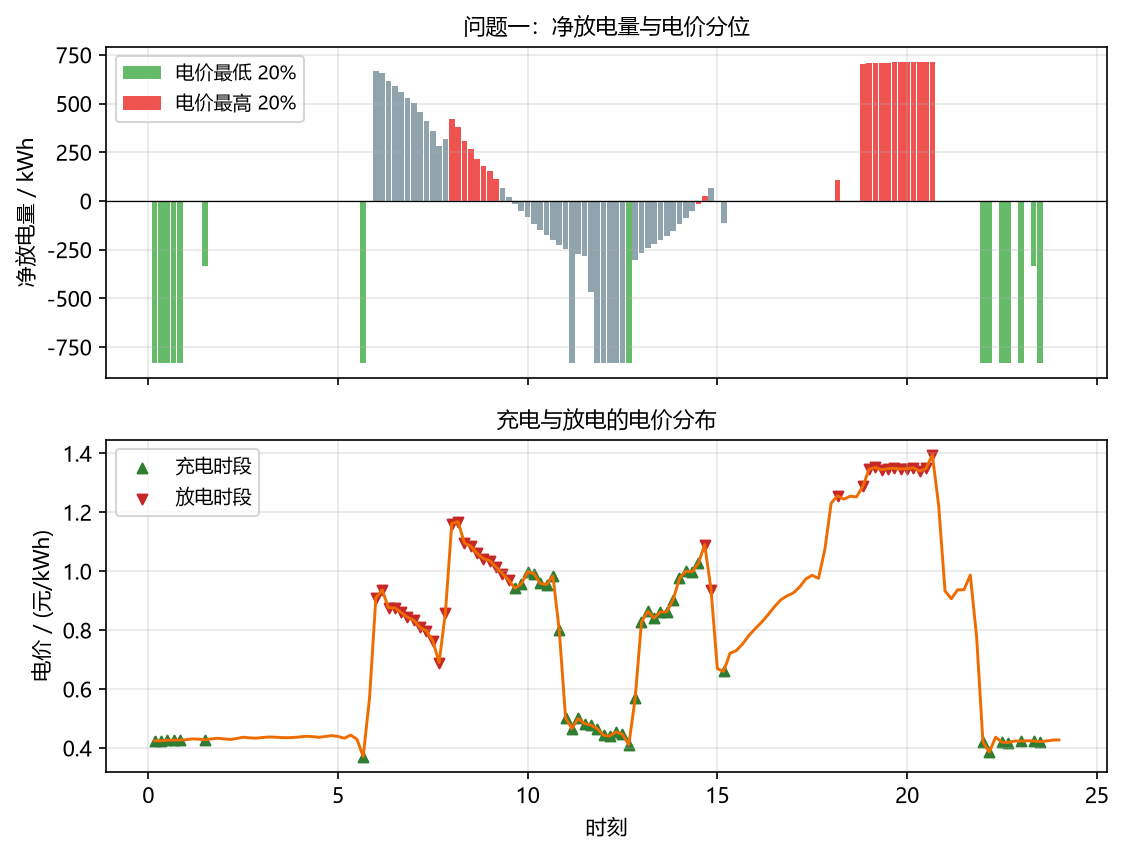
\includegraphics[width=0.490\textwidth]{fig03_p1_arbitrage.png}
\caption{净放电量与电价分位}
\label{fig:p1a}
\end{figure}

\begin{figure}[htbp]
\centering
\begin{minipage}[t]{0.485\textwidth}
\centering
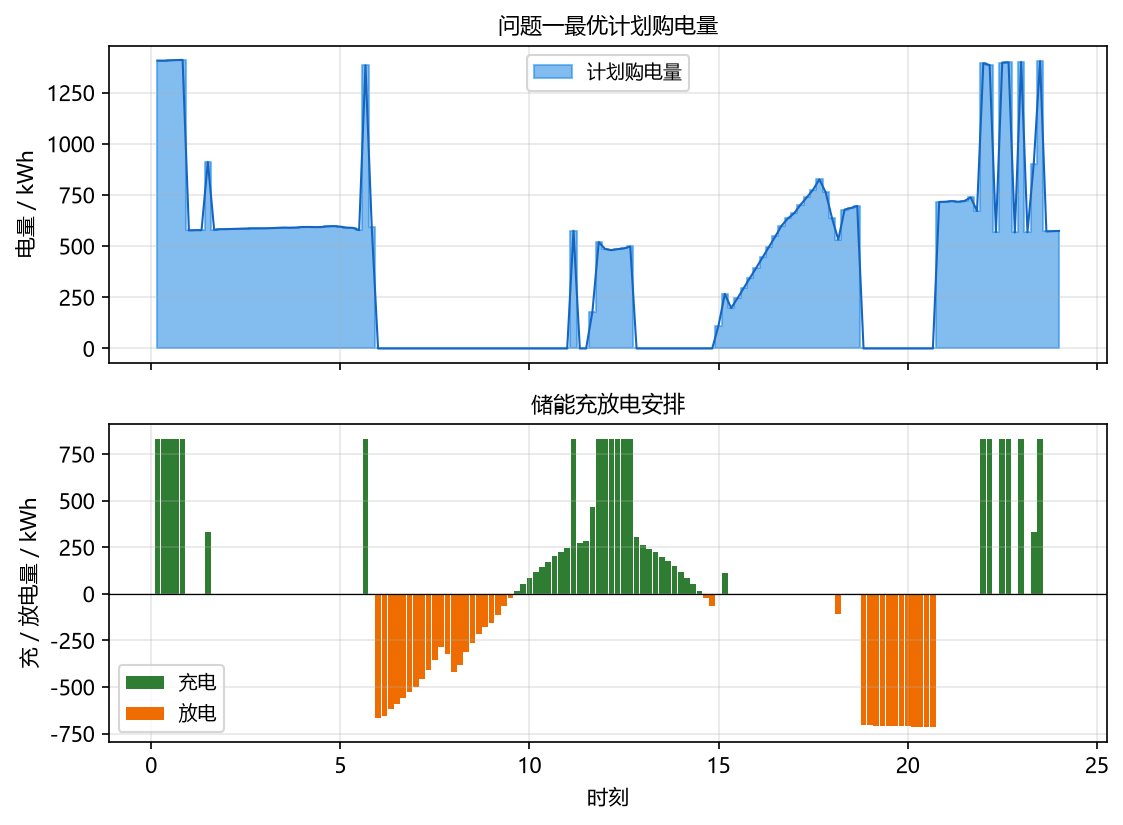
\includegraphics[width=\linewidth]{fig04_p1_dispatch.png}
\caption{问题一最优计划购电量与储能充放电安排}
\label{fig:p1b}
\end{minipage}\hfill
\begin{minipage}[t]{0.485\textwidth}
\centering
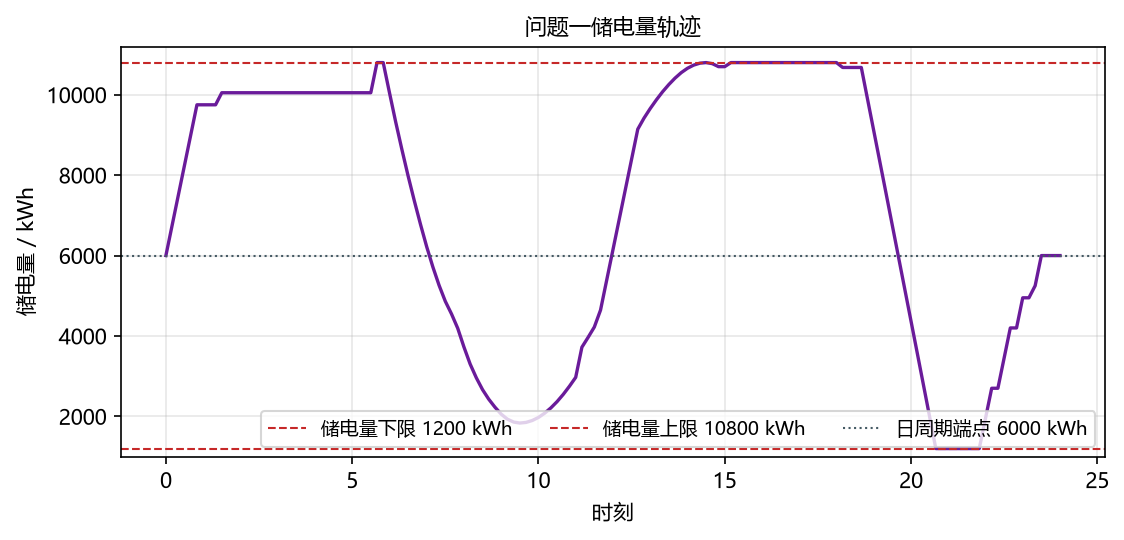
\includegraphics[width=\linewidth]{fig05_p1_soc.png}
\caption{问题一储电量轨迹}
\label{fig:p1c}
\end{minipage}
\end{figure}

\subsubsection{结果检验}

检验从量级、约束与填报三个层次展开。量级上，费用 $35\,126.95$ 元落在独立构造的区间 $[20\,622.73,\,48\,052.05]$ 元内；其中上界 $48\,052.046591$ 元是“完全不使用储能、按分时电价直接购电”的可行策略费用，最优解相对该策略节省 26.898\%，这一比值同时验证了套利的方向与幅度。约束上，68 项独立断言全部通过：功率平衡与状态转移残差为 0，$E_t\in[1200,10800]$，$E_{144}=E_0$，充放电峰值均不越界。填报上，写出的 \texttt{result1.xlsx} 与解序列逐点一致。

\subsubsection{模型族对照}

为确认上述结论不依赖于某一特定建模形式，本文构造了同题的若干变体并逐一求解，结果列于表~\ref{tab:p1ab}。

\begin{table}[htbp]
\centering
\small
\caption{问题一的模型族与建模选择对照}
\label{tab:p1ab}
\begin{tabular}{p{5.4cm}>{\raggedleft\arraybackslash}p{4.6cm}>{\raggedleft\arraybackslash}p{3.6cm}}
\toprule
对照项 & 费用 / 元 & 相对 $C^{*}$ \\
\midrule
基准线性规划（连续松弛） & 35\,126.948589 & $0.000$\% \\
加 144 个互补二元变量的整数模型 & 35\,126.948589 & $0.000$\% \\
储电量离散化 DP（网格步长 400 kWh） & 37\,616.52 & $+7.087$\% \\
储电量离散化 DP（网格步长 200 kWh） & 36\,203.04 & $+3.063$\% \\
储电量离散化 DP（网格步长 100 kWh） & 35\,688.92 & $+1.600$\% \\
储电量离散化 DP（网格步长 50 kWh） & 35\,404.67 & $+0.791$\% \\
去掉日周期约束 & 32\,909.865256 & $-6.312$\% \\
删除弃光变量 & 35\,126.948589 & $0.000$\% \\
效率作用位置：仅充电侧计效 & 33\,416.53 & $-4.869$\% \\
效率作用位置：仅放电侧计效 & 34\,168.61 & $-2.728$\% \\
效率作用位置：往返整体计效 & 33\,801.50 & $-3.773$\% \\
\bottomrule
\end{tabular}
\end{table}

三点值得强调。其一，加入 144 个互补二元变量的混合整数模型给出的目标值与线性规划\textbf{完全相同}（最优间隙为 0、仅 1 个节点），说明连续松弛在本问上无损，无需付出整数变量的计算代价。其二，储电量离散化的动态规划在四档网格上的目标值恒不低于 $C^{*}$，且随网格加密单调收敛（最细网格偏差 $+0.791\%$），差异来自离散化本身而非模型结构。其三，日周期约束的经济价值为 $2217.083333$ 元，占 $C^{*}$ 的 6.312\%：去掉该约束后模型会把期末库存放空至下限，相当于把日初存量的电能当日变现。这说明“0:00 与 24:00 储电量相同”并非形式要求，而有实质经济含义，也是问题二允许跨日携带电量后费用结构变化的根源。

效率作用位置的三组对照（仅充电计效、仅放电计效、往返整体计效）所得费用比统一处理方式低 958--1710 元，表明本文采用的“充放两侧各按 90\% 计”是几种可能处理方式中最保守的一种。附录给定的 90\% 是题面硬参数；实际电池效率随荷电状态与老化变化，恒效率属工程简化\cite{ref-vykhodtsev-2022-bess-review,ref-huang-2022-dynamic-efficiency}。目标中不计折旧同样是显式取舍——日前微网调度文献常把退化成本纳入目标\cite{ref-zhang-2015-dayahead-degradation}，题面未给相应系数，故本文在假设中声明而不隐藏。

\subsubsection{稳健性}

在 948 个情景（947 个可行）的扰动实验下，问题一的结论判为“稳定”，全部检验标准通过。费用对往返效率最敏感且方向单调：$\eta$ 由 0.9 降至 0.8 时费用上升 8.885\%，升至 1.0 时下降 7.828\%，弹性约为 $-0.70$ 至 $-0.80$；其余参数的影响均不超过 0.7\%，其中初始储电量在 $[3000,9000]$ kWh 内的变化对费用影响不超过 0.07\%——日周期闭合使初值只影响日内可调度裕度，不影响总量。噪声实验显示费用区间半宽不超过 11.6\%，且均值存在负向偏移，该偏移源于价格函数的凹性，不应解读为预测误差可以省钱。

\subsection{问题二：全年计划购电策略与紧急购电}

\subsubsection{模型的建立}

问题二去掉日周期约束，把决策期扩展到全年 365 天，并用跨日状态连续性取代它：

\begin{equation}
E_{d,0}=E_{d-1,144},\qquad E_{1/1,0}=6000,\qquad E_{12/31,144}\ \text{自由}
\end{equation}

式 (10) 就是状态转移式在日边界处的一次转移，不需要额外约束。与问题一相比的关键差别在于：储能在不同日期之间可以携带电能，因此“哪天充电、哪天放电”也成为决策的一部分；目标中新增紧急购电项 $\alpha_{em}p_{\tau}q^{em}_{\tau}$，$\alpha_{em}=5$。把跨日时段统一为一个长时域优化问题，是微网与储能调度中处理日间耦合的标准做法\cite{ref-silvente-2015-rolling-horizon,ref-holjevac-2017-receding-horizon,ref-hu-2020-mpc-overview,ref-finnah-2021-da-intraday-adp}。

\subsubsection{紧急购电恒为零的条件与意义}

\begin{quote}
\textbf{定理 2（紧急购电的机制性恒零）} 若 ① 电价 $p_{\tau}>0$；② $\alpha_{em}>1$；③ 计划购电量 $b_{\tau}$ 无上界；④ 计划层对当日负载与光伏为完全信息，则模型存在满足 $q^{em}_{\tau}\equiv0$ 的最优解。

\textbf{证明} 设某时段 $q^{em}_{\tau}=\delta>0$。由于平衡为等式且 $b_{\tau}$ 无上界，把该时段计划购电量改为 $b'_{\tau}=b_{\tau}+\delta$ 仍可行（平衡方程左端不变），而费用变化为 $p_{\tau}\delta-\alpha_{em}p_{\tau}\delta=p_{\tau}\delta(1-\alpha_{em})<0$，即费用严格下降，与最优性矛盾。故存在最优解使 $q^{em}\equiv0$。$\square$
\end{quote}

定理 2 说明：在完全信息且购电无上限的口径下，紧急购电惩罚机制\textbf{不会}被激活，交付表中紧急购电量全零是模型结构的推论，而非数据巧合。这一点必须在论文中解释清楚，否则“表格全零”会被误读为漏填。同时也说明该机制不可删除：一旦引入购电功率上限，紧急购电立即被激活，本文用上限扫描给出激活阈值——限额压到 4218.75 kW 时全年紧急购电量升至 8707.398542 kWh 并涉及 14 天，压到 2000 kW 时升至 7\,845\,369.336456 kWh 并涉及全部 365 天，总费用单调上升至 2.38 倍。因此“无上限”是必须显式声明的前提，而非可以省略的细节。文献亦普遍强调：日前决策与实时结算之间的信息落差与功率约束是应急机制被激活的直接原因\cite{ref-chazarra-2017-perfect-information,ref-toubeau-2020-da-real-time,ref-vanderveen-2016-balancing-market-design,ref-herre-2020-imbalance-settlement,ref-joos-2018-integration-costs}。

\subsubsection{主结果}

全年最优购电费为 $13\,758\,182.573724$ 元，其中交付期（2025 年 2 月 1 日--12 月 31 日，334 天）为 $12\,233\,050.830708$ 元，1 月预热期为 $1\,525\,131.743016$ 元，三者满足“交付期加预热期等于全期”的加总关系。主要总量指标列于表~\ref{tab:p2main}。

\begin{table}[htbp]
\centering
\small
\caption{问题二的主要结果}
\label{tab:p2main}
\begin{tabular}{lll}
\toprule
指标 & 数值 & 口径与说明 \\
\midrule
总购电费（全期 365 天） & 13\,758\,182.573724 元 & 交付期 334 天为 12\,233\,050.830708 元，1 月预热期 1\,525\,131.743016 元 \\
紧急购电费 & 0 元 & 由定理 2 保证 \\
计划购电量 $\sum b$ & 22\,657\,938.157435 kWh & 全期 \\
充电量 $\sum c$ / 放电量 $\sum q^{dis}$ & 7\,364\,620.676347 / 5\,969\,662.747841 kWh & 往返损耗 19\% \\
弃光量 $\sum s$ & 990\,168.090312 kWh & 97 天出现弃光，全部落在交付期 \\
净负荷 $N$ & 20\,272\,812.138617（全期）/ 17\,939\,189.494967（交付期）kWh & 与价格无关，用于跨问题校验 \\
储电量端点 & $E_{2/1,0}=7950.000000$，$E_{12/31,144}=1200.000000$ kWh & 跨日滚动、终端自由 \\
\bottomrule
\end{tabular}
\end{table}

量级自检方面，费用落在独立构造的区间 $[7\,525\,691.131,18\,298\,592.366]$ 元内；套利方向正确，充电加权均价 0.520371 元/kWh 明显低于放电加权均价 1.154986 元/kWh。储电量两端（1200 与 10800 kWh）在最优解中均曾活跃，最大购电量出现在功率上限处，峰值购电功率约 10325.33 kW。

\subsubsection{交付结果}

表~\ref{tab:p2a} 给出题面四个指定日期的六个 10 分钟时段购电量、全天购电量与全天购电费；表~\ref{tab:p2b} 给出这四个日期的分块充放电量。四个日期及全年的紧急购电量均为 0，按填报口径在“紧急购电量”工作表中逐日填“—/0”、每日至少一行。需特别提醒：题面表 4 中的 2025 年 3 月 1 日及三个时段是\textbf{填写格式示例，不是本题答案}。

\begin{table}[htbp]
\centering
\small
\caption{问题二：四个指定日期的指定时段购电量与全天合计（单位：kWh；购电费单位：元）}
\label{tab:p2a}
\begin{tabular}{lrrrrrrrr}
\toprule
日期 & 10:00 & 12:00 & 14:00 & 16:00 & 18:00 & 20:00 & 全天购电量 & 全天购电费 \\
\midrule
2025-03-20 & 0.00 & 558.311667 & 0.00 & 507.324167 & 682.353333 & 0.00 & 61\,658.562881 & 37\,975.400853 \\
2025-06-21 & 0.00 & 0.00 & 0.00 & 27.005000 & 385.901667 & 0.00 & 38\,934.072483 & 20\,470.622813 \\
2025-09-23 & 0.00 & 380.021250 & 0.00 & 493.582500 & 752.645000 & 61.911667 & 66\,265.421309 & 41\,351.897551 \\
2025-12-21 & 0.00 & 906.683333 & 0.00 & 795.930417 & 712.633333 & 30.268333 & 93\,770.214940 & 59\,717.364845 \\
\bottomrule
\end{tabular}
\end{table}

\begin{table}[htbp]
\centering
\footnotesize
\caption{问题二：四个指定日期的分块充放电量（单位：kWh；块顺序为 0--4、4--8、8--12、12--16、16--20、20--24 时）}
\label{tab:p2b}
\begin{tabular}{llrrrrrrl}
\toprule
日期 & 量 & 第 1 块 & 第 2 块 & 第 3 块 & 第 4 块 & 第 5 块 & 第 6 块 & 端点储电量 0:00 $\to$ 24:00 \\
\midrule
2025-03-20 & 充电 & 1666.67 & 833.33 & 6291.46 & 4689.68 & 0.00 & 3503.18 & \multirow{2}{*}{8550.00 $\to$ 4352.87} \\
 & 放电 & 0.00 & 5862.62 & 2777.38 & 254.72 & 5728.06 & 2911.94 & \\
2025-06-21 & 充电 & 0.00 & 833.33 & 701.60 & 9965.07 & 0.00 & 8166.67 & \multirow{2}{*}{2361.06 $\to$ 8550.00} \\
 & 放电 & 0.00 & 1719.95 & 0.00 & 0.00 & 6154.10 & 2485.90 & \\
2025-09-23 & 充电 & 1666.67 & 833.33 & 5245.38 & 5923.78 & 0.00 & 8166.67 & \multirow{2}{*}{8550.00 $\to$ 8550.00} \\
 & 放电 & 0.00 & 6746.77 & 1896.62 & 403.62 & 5640.00 & 3000.00 & \\
2025-12-21 & 充电 & 1666.67 & 1666.67 & 5833.33 & 7574.21 & 0.00 & 8166.67 & \multirow{2}{*}{8550.00 $\to$ 8550.00} \\
 & 放电 & 0.00 & 1425.00 & 7890.00 & 2220.11 & 5797.47 & 2842.53 & \\
\bottomrule
\end{tabular}
\end{table}

这里必须区分两种端点语义：问题一的 0:00 与 24:00 是\textbf{日周期约束}的端点，恒为 6000 kWh；问题二的端点是全年滚动轨迹在某一日的切片，随日期变化，两者不可直接比较。

\subsubsection{策略形态与机制解释}

问题二的最优策略在更长时间尺度上重复了套利逻辑，但也出现两个新现象（图~\ref{fig:p2a}）。

第一，\textbf{储能存在明显的“回归水平”}：334 个交付日中，日初或日末储电量等于 8550.00 kWh 的各有 219 天，全年日初储电量只取 96 个不同水平。这说明最优策略倾向于把储能维持在高位以待高价时段，而不是每天放空再充满；只有 12 月 31 日（决策期最后一天）日末落到下限 1200 kWh，即期末放空，对应式 (8) 中 $-4320$ kWh 的库存变现项。

第二，\textbf{弃光只发生在少数日子}：全期仅 97 天出现弃光，合计 990168.090312 kWh，占光伏总发电量的比例很小。这说明在无售电收益的设定下储能容量基本足以吸收盈余；但弃光变量仍必须保留，否则那些盈余超过储能吸收能力的时段会使模型不可行。

策略形态的统计量为：电价与充电量的相关系数 $-0.3835$，与放电量的相关系数 $+0.6132$；最便宜的 20\% 电价时段承担 48.12\% 的充电量，最贵的 20\% 时段承担 68.42\% 的放电量；交付期单日费用最小 11\,900.552329 元、最大 60\,014.368886 元、均值 36\,625.900691 元（合计与交付期费用逐位一致）。

\begin{figure}[htbp]
\centering
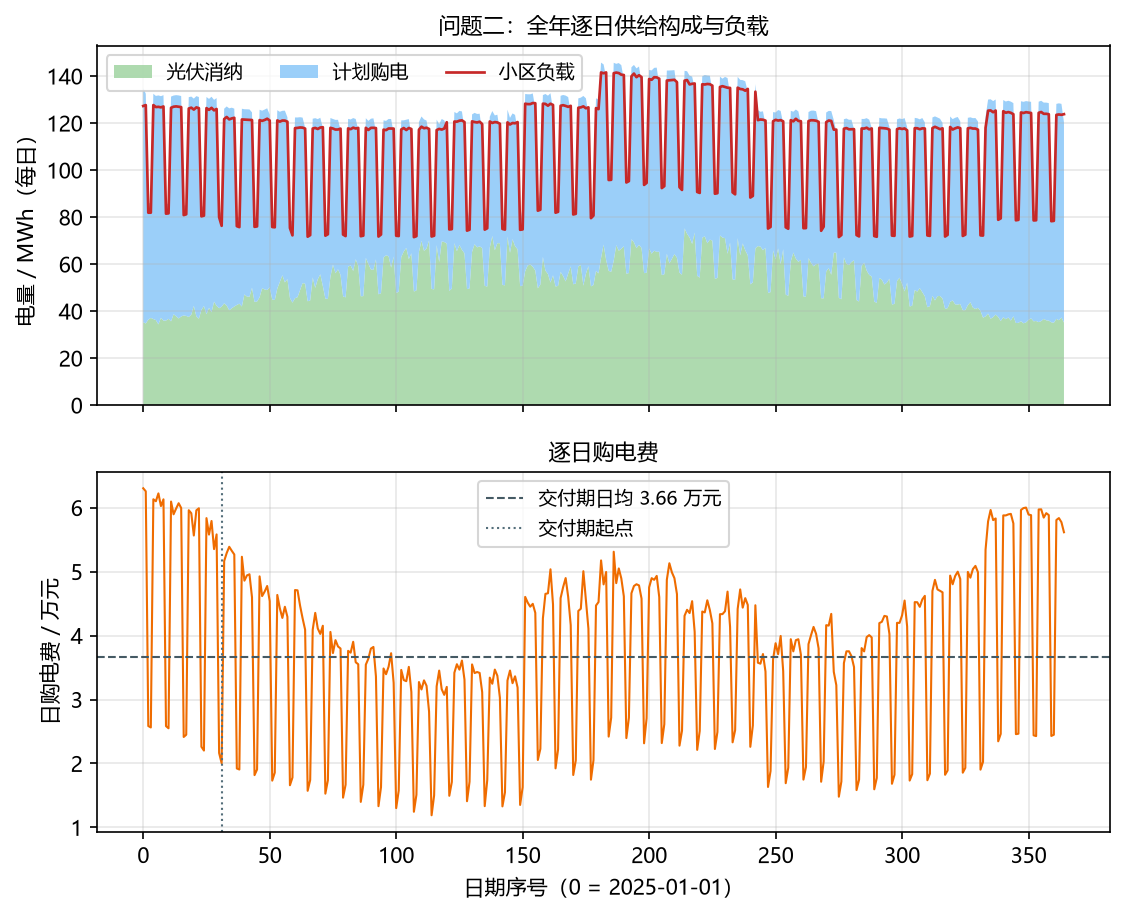
\includegraphics[width=0.80\textwidth]{fig06_p2_energy_flow.png}
\caption{全年逐日供给构成、负载与逐日购电费}
\label{fig:p2a}
\end{figure}

\begin{figure}[htbp]
\centering
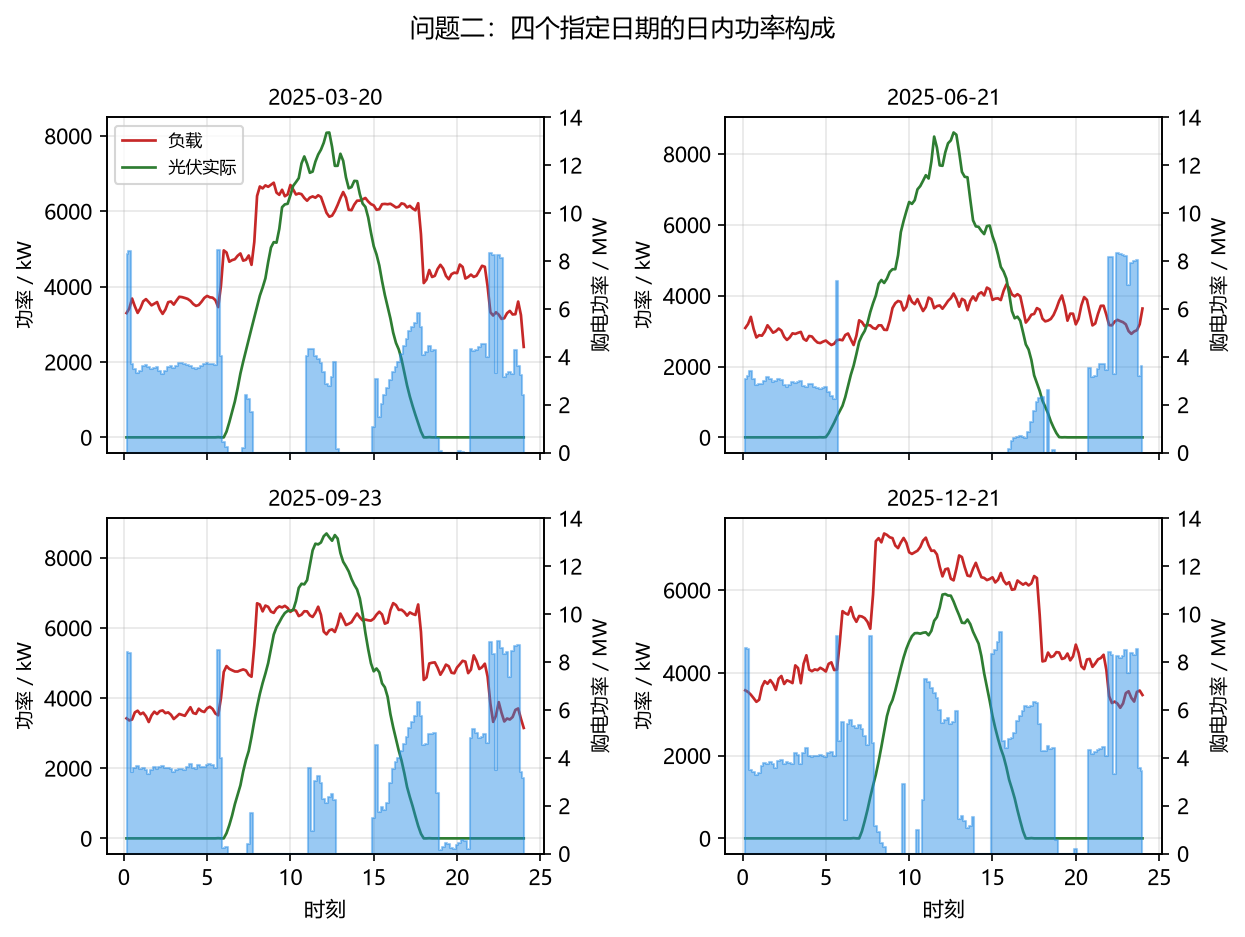
\includegraphics[width=0.80\textwidth]{fig08_p2_spec_dates.png}
\caption{题面四个指定日期的日内功率构成}
\label{fig:p2c}
\end{figure}

\subsubsection{模型族与结构对照}

本文设置了 17 组对照（表~\ref{tab:p2ab}），结论有三点。

其一，\textbf{核心结论不依赖模型族与实现路线}。用不同变量排序、消去弃光变量、改用对偶单纯形法的独立第二实现给出的费用与主模型逐位相同；把全年问题精确分解为 365 个单日问题（耦合量取全年最优值）也给出相同结果。差异为零说明主结果不是实现假象。

其二，\textbf{跨日与终端口径有可量化的经济价值}。逐日解耦并允许日终自由递推会使费用上升 26\,894.74 元，这是“跨日携带电能”的价值；逐日施加日周期约束会使费用上升 17\,135.02 元，这是跨日衔接与逐日终端两项的\emph{合并}贡献；把全年终端固定为 6000 kWh 会使费用上升 2217.08 元，对应期末放空的 4320 kWh 库存。三者对应不同的约束改动，不可互相替代或相加。

其三，\textbf{购电上限是唯一能激活紧急购电的机制}（图~\ref{fig:p2d}）。上限在 10326 kW 及以上时不产生任何影响（该值只是“非绑定阈值”），而在 4218.75 kW 及以下时紧急购电被激活且费用随上限下降单调上升，代价从 $+694\,101$ 元迅速放大到 $+19\,011\,429$ 元（上限 2000 kW）。这说明“紧急购电为零”的结论对上限极度敏感，必须与前提条件一并陈述。

\begin{table}[htbp]
\centering
\small
\caption{问题二的时域组织、终端条件与购电上限对照（费用为全期，单位：元）}
\label{tab:p2ab}
\begin{tabular}{p{7.0cm}rr}
\toprule
对照项 & 费用 & 相对基准 \\
\midrule
基准（全年单一长时域 LP） & 13\,758\,182.573724 & --- \\
独立第二实现 / 精确逐日分解 & 13\,758\,182.573724 & $+0.000000\%$ \\
逐日解耦、日终自由递推 & 13\,785\,077.313742 & $+0.195482\%$ \\
逐日施加日周期约束 / 终端固定为 6000 kWh & 13\,775\,317.596266 / 13\,760\,399.657058 & $+0.124544\%$ / $+0.016115\%$ \\
购电上限 4375 / 4218.75 / 2000 kW & 14\,452\,283.680247 / 14\,647\,566.902931 / 32\,769\,611.572155 & $+5.045\%$ / $+6.464\%$ / $+138.183\%$ \\
互补约束整数模型（52\,560 个二元变量） & 13\,758\,186.928903 & $+0.000032\%$ \\
\bottomrule
\end{tabular}
\end{table}

\begin{figure}[htbp]
\centering
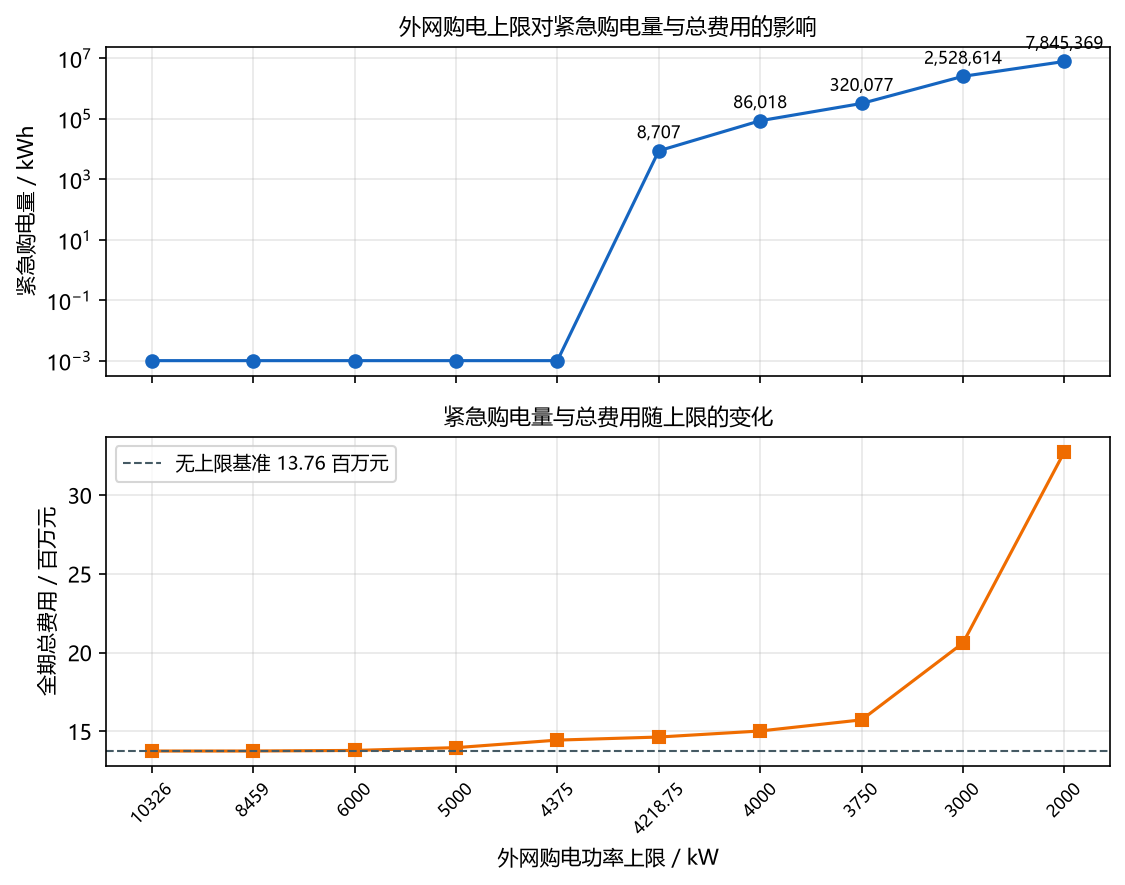
\includegraphics[width=0.80\textwidth]{fig09_p2_bcap.png}
\caption{外网购电上限对紧急购电量与总费用的影响：上限降至 4218.75 kW 及以下时紧急购电被激活}
\label{fig:p2d}
\end{figure}

\subsubsection{稳健性与适用边界}

149 次全年线性规划的扰动实验得到两点结论（判据与阈值在跑数前冻结）。第一，\textbf{年度与交付期总量稳健}：参数扰动下费用最大偏移 14.078\%（对应 $\eta=0.72$ 的极端档），噪声情景下费用区间半宽不超过 0.96\%，全部情景可行、无 NaN 或无穷值。第二，\textbf{日尺度交付量对效率口径敏感}：$\eta$ 变化 $\pm10\%$ 可使单日购电量与购电费移动约 $\pm20\%$（实测最大 19.62\%），而年度总量仅移动约 $\pm7\%$。因此表~\ref{tab:p2a}、表~\ref{tab:p2b} 中的单日数值须与该敏感性一并引用。

本文如实登记两条未通过的判据。其一，可行率判据的唯一失败样本来自求解器设置对照，其目标值与基线\textbf{逐位相同}、约束残差为 $2\times10^{-12}$、解可行，唯一未通过的检查是“返回解是否满足充放电互补性”——由于引理 1 只断言\emph{存在}互补最优解而非任意返回解都互补，这属于退化最优面上的返回解选择问题，不构成模型不可行。其二，交付表稳定判据的失败样本来自 $\eta=0.99$ 的情景，该情景使 2025 年 6 月 21 日全天购电量下降 19.10\%，属\emph{有利方向}的变化，但因判据取绝对值口径而被判失败；其反向（$\eta=0.81$）最多使单日购电费上升 12.97\%，有 21 天升幅超过 10\%。据此本问的稳定性分级为“脆弱（需缩小适用范围）”，判据未做事后修改。

此外登记两项属于结构性口径的发现：一是当允许以 0.50 元/kWh 售电时，松散的弃光上界会出现“售出电量超过物理盈余”的非物理套利（售出 5\,845\,778.709901 kWh 远超物理盈余 3\,120\,221.003233 kWh），须先收紧上界，该情景收益不得当作真实售电收入；二是当把紧急购电倍数改为 0.5 时全年紧急购电量恰等于基准的全年计划购电量，这是同一物理计划被整体改记为紧急购电的“重标定效应”，不得把它解读为净负荷。

\subsection{问题三：光伏预报、多时刻调整与偏差分段结算}

\subsubsection{问题分析}

问题三在问题二的基础上引入两级信息落差，二者分别触及模型的输入与结构。一是粒度落差：光伏预报只在每天 0:00、6:00、12:00、18:00 发布，且只给整点值，可决策与结算的粒度为 10 分钟，因此必须先把整点预报降到 10 分钟。二是时刻落差：可以按预报调整当天计划，但计划量与调整量之间要按“低于计划只退 0.5 倍价、高于计划需补 1.5 倍价”双向分段结算，因此必须明确在什么时刻、依据什么信息调整。本文据此先明确各决策时刻各自能看到什么，再建立“0:00 计划 + 三个时刻调整 + 事后结算”的三层模型，并保留紧急购电作为最终兜底。

本题很容易被忽略的一点是：调整机制并非没有代价。它减少了紧急购电，却引入了偏差违约金，二者孰大孰小只能由定量结果回答——这正是后文给出费用分项的原因。

\subsubsection{预报降尺度与信息集}

本文的做法是：把“预报 $k$ 小时”解释为发布时刻 $m$ 之后第 $k$ 个整点的功率点值；时段 $i$ 的左端点落在小时区间 $[h,h+1)$ 时取 $P(h)$ 与 $P(h+1)$ 的线性插值；发布时刻之后的第一小时无左端整点值，用 $P(m+1)$ 前向保持。把小时级预报细化到分钟级的插值方法及其对调度结果的影响在相关文献中已有系统讨论\cite{ref-almpantis-2024-minute-downscaling,ref-barbieri-2017-very-short-term-pv,ref-stenzel-2016-temporal-resolution}。

该做法有两个必须说明的性质。其一，\textbf{不强制块内能量守恒}：整点锚定线性插值得到的块内平均功率为 $(2.5A_{k-1}+3.5A_k)/6$，一般不等于 $A_k$，因此降尺度会系统性地改变能量。其二，\textbf{跨年项不消费}：$m=6,12,18$ 时分别有 19--24、13--24、7--24 小时的预报落在次日之后，合计 36 项被丢弃，本文不做截断也不做外推。这两点的影响在模型族对比中单独量化。

信息集按“模型假设”一节的非预期性约定逐层落实，此处只补充两点实现后果：附件 2 的实际光伏只进入事后结算层，不进入任何决策层；时段 $i$ 由唯一一个决策时刻支配，记为 $\nu(i)=6\lfloor(i-1)/36\rfloor$，无需引入离散选择变量，模型保持线性。

\subsubsection{三层模型的建立}

按时间顺序组织模型为三层，逐层求解、逐层提交，不允许用一次性联合优化让前两层“看到”实际光伏。

\textbf{计划层（0:00）}使用 0:00 预报的全天光伏轨迹 $\Pi_0[PV]$，求解

\begin{equation}
\min_{b,\,c,\,q^{dis},\,s,\,E}\ \sum_{i=1}^{144}p_ib_i
\quad\text{s.t.}\quad
b_i+\Pi_0[PV]_i\Delta t+q^{dis}_i=L_i\Delta t+c_i+s_i
\end{equation}

外加储能动态、容量与功率约束；储电量在日边界衔接上一日已提交的末态，全年终端自由。

\textbf{调整层（6:00、12:00、18:00）}以当天 0:00 的计划量 $b$ 为参数，只决定其支配时段的最终购电量 $q$，目标为该层剩余时段上的偏差惩罚：

\begin{equation}
\min\ \sum_{i\in R_m}\Bigl[\beta_{def}\,p_i\,\bigl(b_i-q_i\bigr)^{+}+\beta_{over}\,p_i\,\bigl(q_i-b_i\bigr)^{+}\Bigr],
\qquad \beta_{def}=0.5,\ \ \beta_{over}=1.5
\end{equation}

其中 $(x)^+=\max(x,0)$，实现时用两个非负辅助变量分段线性化，因系数为正故线性松弛无损；调整层初值取实际已实现的储电量，已提交时段不再修改。这类“滚动调整 + 双向偏差惩罚”的多阶段结构在日内再调度与偏差结算文献中被广泛采用\cite{ref-li-2016-two-stage-rhc,ref-bhattacharya-2018-multistage-storage,ref-elkazaz-2020-convex-mpc-rhc,ref-danti-2019-intraday-rescheduling,ref-matsumoto-2022-imbalance-design,ref-asgarpoor-1995-deviation-penalty}。

\textbf{实际结算层}在全部决策提交后事后计算，是附件 2 实际光伏的唯一入口。设剩余量 $r=q+q^{dis}+PV^{act}\Delta t-L\Delta t-c$，则

\begin{equation}
s'=\max(0,r),\qquad q^{em}=\max(0,-r)
\end{equation}

\begin{equation}
C_{\text{plan}}=\sum p b,\quad
C_{\text{adj}}=\sum\Bigl[\beta_{def}p(b-q)^{+}+\beta_{over}p(q-b)^{+}\Bigr],\quad
C_{\text{em}}=\sum \alpha_{em}p\,q^{em}
\end{equation}

其中 $b$ 是计划购电量、$q$ 是最终购电量（替代量的含义），二者不可混用。

\subsubsection{主结果与交付结果}

交付期总费用为 $14\,540\,616.335652$ 元，构成为：计划购电费 $12\,362\,860.209641$ 元、调整结算费 $510\,208.940910$ 元、紧急购电费 $1\,667\,547.185102$ 元（全期三项分别为 $13\,885\,669.475555$、$563\,098.132533$、$1\,730\,408.537141$ 元）。费用落在独立构造的区间 $[6\,963\,514.20,16\,407\,319.63]$ 元内，自下界起位于 80.23\% 处；交付期均价 0.697655 元/kWh，落在最小电价与 5 倍最大电价之间。交付期紧急购电量 391\,274.485914 kWh、弃光量 2\,087\,727.847547 kWh、最终购电量 $\sum q=20\,842\,142.600809$ kWh（注意该值不是计划购电量 $\sum b=20\,359\,871.873818$ kWh）。

表~\ref{tab:p3a} 给出四个指定日期的全天费用及其分项与紧急购电的合并区间数和合计电量。四个日期的 0:00 与 24:00 储电量均为 1200.000000 kWh，充放电量按 4 小时块分别列示、不做冲抵。同样提醒，题面表 4 中的 2025 年 3 月 1 日及其区间为格式示例。

\begin{table}[htbp]
\centering
\small
\caption{问题三：四个指定日期的全天购电量、购电费分项与紧急购电结构（日期为列、指标为行，单位随各行标注）}
\label{tab:p3a}
\begin{tabular}{lrrrr}
\toprule
指标 & 2025-03-20 & 2025-06-21 & 2025-09-23 & 2025-12-21 \\
\midrule
全天购电量 $\sum q$ / kWh & 70\,040.887993 & 33\,532.164963 & 68\,433.174470 & 94\,749.308713 \\
全天购电费 / 元 & 52\,814.209286 & 22\,848.629380 & 47\,936.179117 & 62\,365.864792 \\
\quad 其中计划购电费 / 元 & 41\,095.385464 & 18\,055.815827 & 42\,772.756895 & 59\,764.834892 \\
\quad 其中调整结算费 / 元 & 2\,373.895890 & 1\,088.445153 & 0.000000 & 1\,182.684937 \\
\quad 其中紧急购电费 / 元 & 9\,344.927933 & 3\,704.368400 & 5\,163.422222 & 1\,418.344963 \\
\midrule
紧急购电合并区间数 / 天 & 5 & 7 & 9 & 8 \\
紧急购电量合计 / kWh & 2062.489153 & 840.356133 & 1150.194481 & 352.514922 \\
\bottomrule
\end{tabular}
\end{table}

\subsubsection{机制解释}

\textbf{调整费全部来自超发方向。} 式 (14) 中欠发方向费用为 $0.0$ 元、超发方向为 563\,098.132533 元，即全部调整成本来自“最终购电量高于计划”的时段（上调 5810 个时段、下调仅 86 个时段）。原因是计划层只看 0:00 预报而结算层使用实际光伏：预报低估光伏时计划量偏高（对应下调），高估时偏低（对应上调），实测以后者为主。这一不对称是本文刻意保留的：计划层的目标只含计划费用，不引入对紧急购电的预期，以保证与题面“根据 0:00 预报制定计划”的语义一致。

\textbf{紧急购电非零的成因是预报误差，而非购电上限。} 决策层用附件 3 预报、结算层用附件 2 实际值，二者的差异必然在结算层造成缺口，由 5 倍价的紧急购电补足，交付期合计 391\,274.485914 kWh。本问不设购电功率上限，紧急购电并非“上限被顶到”所致。

\textbf{问题三比问题二更贵，这是一个必须说明的结论。} 两问交付期净负荷\textbf{逐位相同}（17\,939\,189.494967 kWh），而交付期费用分别为 $14\,540\,616.34$ 元与 $12\,233\,050.83$ 元，差额为

\begin{equation}
2\,307\,565.50\ \text{元}\quad(+18.863\%)
\end{equation}

构成为紧急购电费 1\,667\,547.185102 元加调整费 510\,208.940910 元，本质是“预报误差的代价”。本文据此明确指出：\emph{问题三并不比问题二更省}。模型之所以没有抵消这一代价，是因为计划层的目标 $\min\sum p\,b$ 只看 0:00 预报、对紧急购电没有任何预期，模型内部缺少对冲机制；这一事实同时构成了后文讨论“是否需要引入随机优化”的必要性证据。

\textbf{日边界储电量恒为下限，且这是结构性结果而非题面要求。} 全年 365 天的 $E_{d,144}$ 全部等于 1200 kWh，唯一取值数为 1（图~\ref{fig:p3soc}）。题面只在问题一要求“0:00 与 24:00 储电量相同”，本问没有该要求；该现象源于“计划层为单日线性规划 + 目标只含计划费用 + 终端自由”这一组合使跨日库存的边际价值为零，属结构性涌现结果，不应表述为模型缺陷，也不应表述为“题面要求每天放空”。需要注意的是，日边界归零并不等于储能闲置：时段级解序列显示每个交付日内的储电量都覆盖了整个运行区间 $[1200,10800]$ kWh（日内极差中位数 9600 kWh），即储能仍在满量程吞吐，只是每日末回到下限。此外，2025 年 2 月 1 日 0:00 的储电量在本问为 1200.00 kWh、在问题二为 7950.00 kWh，差异源于两问信息集不同（问题二用实际值、本问为预报驱动的三层滚动），二者不可直接比较。

\begin{figure}[htbp]
\centering
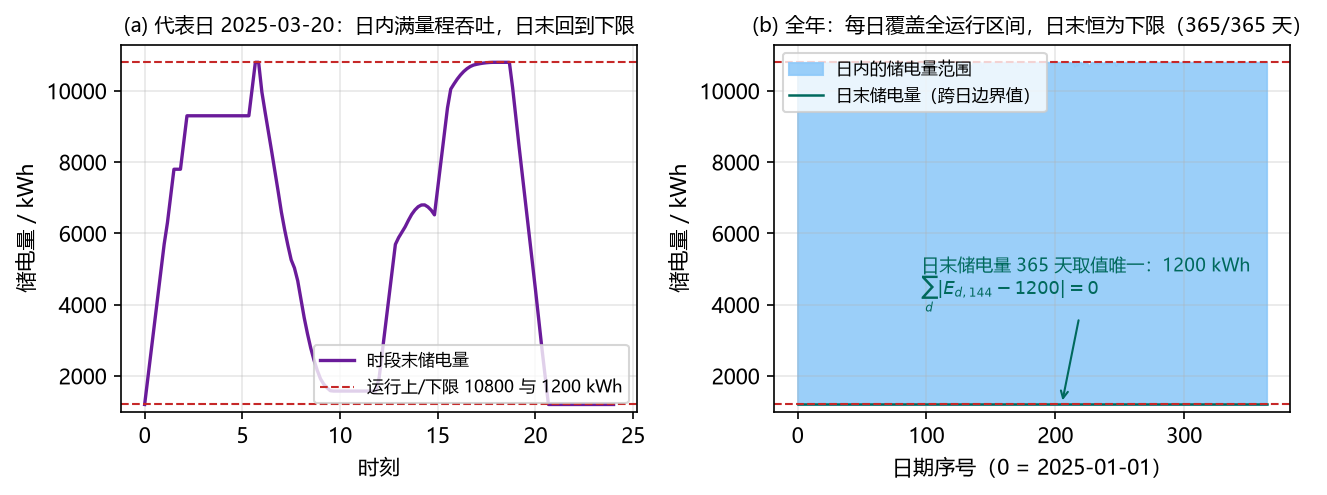
\includegraphics[width=\linewidth]{fig13_p3_soc.png}
\caption{问题三日内储电量行为：(a) 代表日的满量程吞吐与日末回落到下限；(b) 全年每日覆盖全运行区间、日末恒为下限（365/365 天）}
\label{fig:p3soc}
\end{figure}

\begin{figure}[htbp]
\centering
\begin{minipage}[t]{0.485\textwidth}
\centering
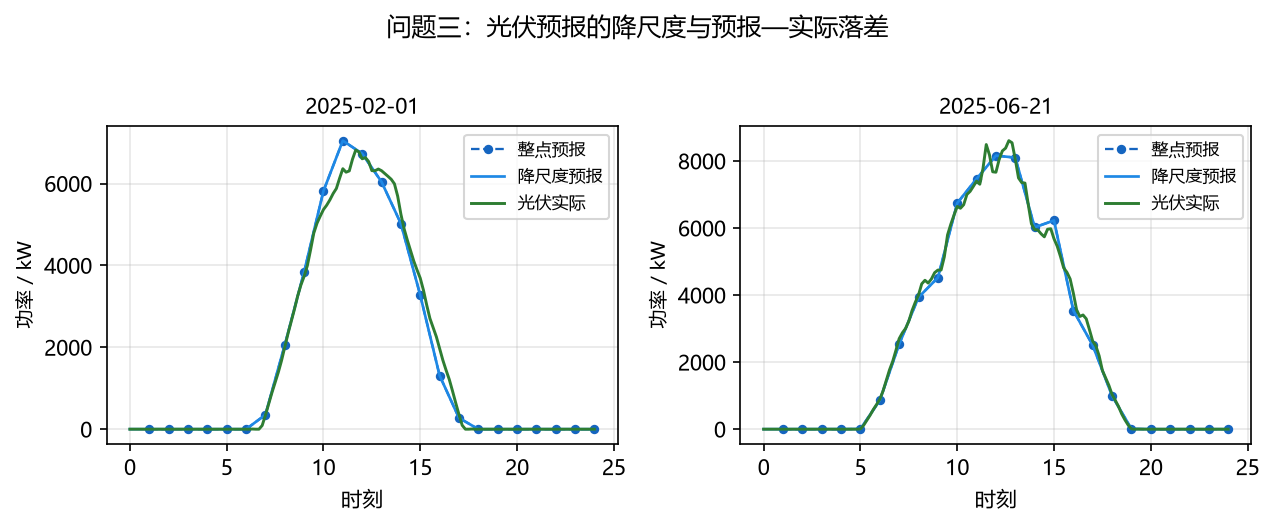
\includegraphics[width=\linewidth]{fig10_p3_forecast.png}
\caption{光伏预报的降尺度与“预报—实际”落差}
\label{fig:p3a}
\end{minipage}\hfill
\begin{minipage}[t]{0.485\textwidth}
\centering
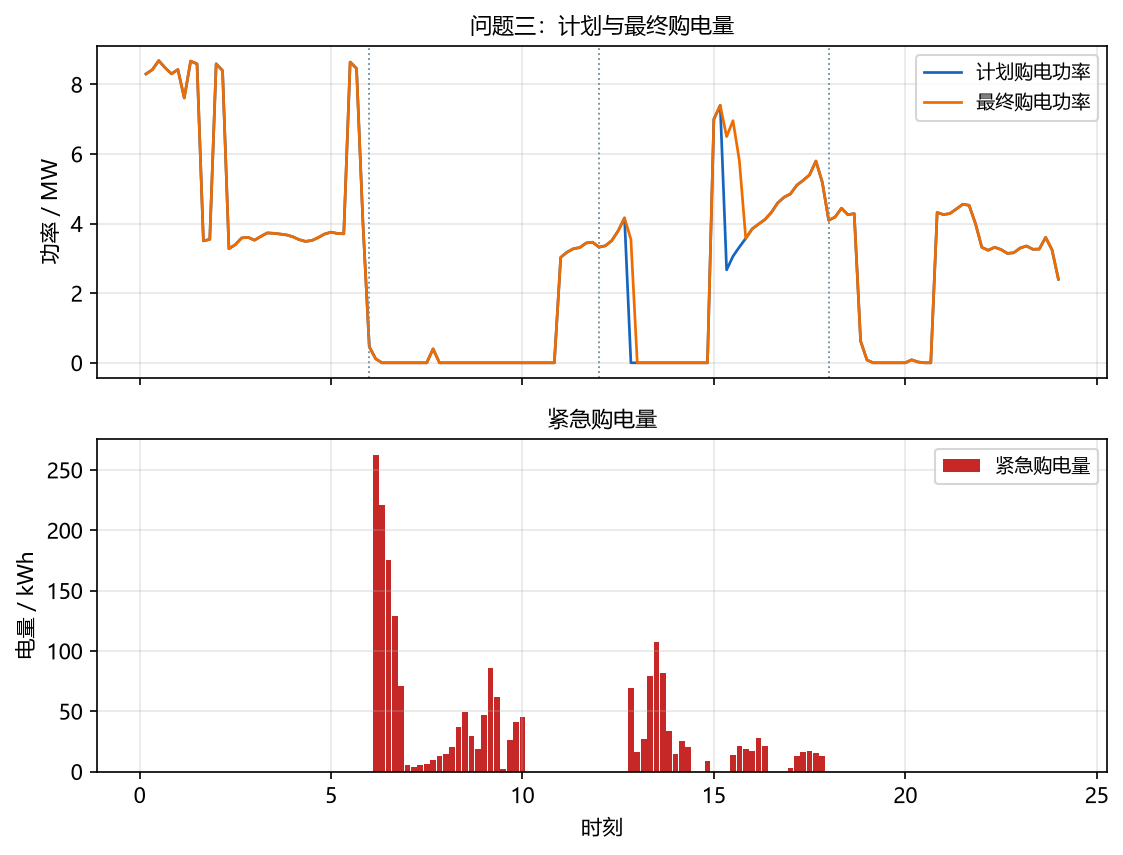
\includegraphics[width=\linewidth]{fig11_p3_profile.png}
\caption{计划量、最终购电量与紧急购电量的日内剖面（虚线为三个调整时刻）}
\label{fig:p3b}
\end{minipage}
\end{figure}

\subsubsection{模型族对比与关键建模选择的影响}

12 组对照的结果表明（表~\ref{tab:p3ab}），主结果不依赖实现路线与求解器设置：逐日解耦的重组实现与主模型逐位同值，两组独立第二实现的链级相对差不超过 $2.17\times10^{-5}$（约 350 元）。表中同时列出若干无收益、甚至方向与直觉相反的对照，本文按事先设定纪律如实记录、不作反向解读，各项影响在对应小节的对照表中给出。

\begin{table}[htbp]
\centering
\small
\caption{问题三的模型族与建模选择对照（全期 365 天，单位：元）}
\label{tab:p3ab}
\begin{tabular}{p{6.6cm}>{\raggedleft\arraybackslash}p{3.6cm}>{\raggedleft\arraybackslash}p{4.0cm}}
\toprule
对照项 & 费用 & 相对主模型 \\
\midrule
主模型（三层顺序向前递推 + 闭式结算） & 16\,179\,176.145228 & --- \\
逐日解耦重组实现 & 16\,179\,176.145228 & $0.000000\%$ \\
独立第二实现 & 16\,178\,825.507754 & $-2.17\times10^{-3}\%$ \\
完全信息上界（单一全年 LP） & 13\,758\,182.573724 & $-14.960\%$ \\
仅 0:00 计划、无调整 & 16\,505\,833.062742 & $+2.019\%$ \\
决策加密至每 3 小时 & 16\,179\,575.041038 & $+0.0025\%$ \\
决策加密至每 1 小时 & 16\,179\,766.212646 & $+0.0036\%$ \\
降尺度改为分段常数（前向保持） & 18\,741\,130.202668 & $+15.834\%$ \\
日初复位为 6000 kWh（非物理对照） & 15\,360\,260.582255 & $-5.061\%$ \\
\bottomrule
\end{tabular}
\end{table}

表~\ref{tab:p3ab} 中有三项建模选择的影响需要强调。第一，\textbf{降尺度处理方式的影响大于调整机制本身的价值}：改为分段常数前向保持使费用上升 2\,561\,954.057440 元（$+15.83\%$），其中紧急购电项贡献占 94.7\%，机制是该做法在主导时段低估光伏 2.68\%、在 12:00 预报域低估 11.29\%，从而系统性地制造缺口。第二，\textbf{完全信息上界比主模型低 14.96\%}，这是信息价值的度量，且该上界与问题二的 accepted 结果逐位相同——它同时充当问题三与问题二之间的独立交叉基准，说明两问的取数与时间对齐完全一致。第三，\textbf{调整机制的价值}为 326\,656.917514 元（相对“仅 0:00 计划”），由“减少的 889\,755.05 kWh 紧急购电”与“新增的 563\,098.13 元违约金”共同决定。

\subsubsection{稳健性，以及“是否需要引入其他时刻的预报”}

扰动实验表明：六组参数方向全部不反转，其中往返效率影响最大（单侧最大 10.9715\%），初始储电量对交付期费用\textbf{完全没有影响}（六档差异均为 0.0，已由独立重解逐位复现）；噪声族内部离散度小于 1\%，但期望费用随误差幅度系统性上移（$\sigma=5\%$ 约 $+3.9\%$、$\sigma=10\%$ 约 $+11.2\%$），原因是噪声只扰动结算层实际值而决策层仍使用预报，缺口由单侧紧急购电与非对称双向结算承接。唯一未通过的检验标准是“跨噪声幅度档的族间均值差 7.29\% 超过 3\%”，同幅度档内仅 0.06\%；该检验标准把“族内离散度”与“跨档均值一致性”绑在一起，属检验设计问题，不构成“模型对噪声不稳定”的证据。据此本问分级为“条件稳定（需给出适用边界）”。购电上限的可行分界落在 $(4375,5000]$ kW，终端条件的经济价值为 3325.625002 元（$+0.0228713\%$）。

关于题面“请分析是否需要引入其他时刻的预报制定调整购电策略”，本文的回答限定在\emph{决策频率}层面，并给出三层证据。第一层是“有没有调整”：加入 6:00、12:00、18:00 三个调整时刻可节省 326\,656.92 元（2.02\%），说明调整机制本身有效。第二层是“在四个时刻之上继续加密”：加密到每 3 小时或每 1 小时，费用反而分别上升 398.90 元与 590.07 元，即\textbf{没有可测收益}，而计算时间从 10.5 s 增加到 69.9 s 与 194.8 s。第三层是“新增预报信息量”：附件 3 只在 0:00、6:00、12:00、18:00 发布预报，本文不构造并不存在的输入，因此上述结论\textbf{不覆盖}“若能获得更频繁发布的预报是否有价值”这一问题——那属于信息供给的变化，需要新的数据来源才能回答。综合而言，在现有预报发布条件下，题面给定的四个决策时刻已经足够，无需引入其他时刻。

\subsection{问题四：波动电价下重算两问}

\subsubsection{价格可观测性口径与预测器}

问题四的核心困难不在优化而在\textbf{信息}。附件 4 给出的是 2025 年逐日波动的实时电价，而“实时”意味着：当 0:00 制定当天计划时，当天 144 个时段的电价尚未发生。若把附件 4 直接当作已知输入，就等于假设电价可以被完全预知，这与题面不符，也会把问题四退化为一次“换电价重算”。因此本文明确采用如下口径：

\begin{quote}
\textbf{价格可观测性约定}：0:00 制定当天计划时，当天以及任何未来日的实时电价均不可观测；决策层只能使用历史电价（前一日及更早）与其他已有数据构造预测价；费用结算一律使用附件 4 的实际电价。
\end{quote}

在此约定下，链 \emph{4-3} 的调整层虽然拥有当天已实现时段的信息，6:00、12:00、18:00 时对当日剩余时段的电价\textbf{仍然不可知}，只能用滚动更新的预测；只有结算时才使用实际价。主预测器取“前一日同时段”$\hat p^{(0)}_{d,i}=p^{act}_{d-1,i}$：该预测器不需要估计参数，且与附件 4 的日内形状稳定性相容。为保证结论不依赖预测器选择，本文同时给出“水平 $\times$ 时段”双因子预测器（用最近 7 个可用历史日的日均价作为当日水平、用历史同时段的归一化形状作为日内结构）与“历史同时段均值”预测器作为基准对照。链 \emph{4-3} 的调整层在此基础上做滚动水平校正：

\begin{equation}
\hat p^{(m)}_{d,i}=
\begin{cases}
p^{act}_{d,i}, & i\le 6m\ \text{（已实现，可直接观测）}\\
\kappa_m\,\hat p^{(0)}_{d,i}, & i>6m
\end{cases},
\qquad
\kappa_m=\mathrm{clip}\!\left(A_m/B_m,\,0.5,\,2.0\right),\quad \kappa_0\equiv1
\end{equation}

其中 $A_m$ 为当天截至时刻 $m$ 已实现电价的均值，$B_m$ 为前一日同时段均价；含义是：若当天价格整体高于前一日同日同时段水平，就把剩余时段的预测按比例上调。实测 $\kappa_m$ 的取值区间为 $[0.66233,1.54939]$，从未触及上下界，即校正始终是内点解。实时电价预测与“用预测价做决策、用实际价结算”的分工在电力市场与储值优化文献中已有共识\cite{ref-lago-2018-spot-price-deep-learning,ref-myttenaere-2016-mape-regression,ref-chitsaz-2018-price-forecast-btm-storage,ref-khani-2015-online-adaptive-rtod,ref-staffell-2016-maximising-storage-value,ref-mathaba-2014-price-forecast-benefit,ref-hodge-2018-forecast-value-storage}。

预测器的滚动回测结果（只用被测日之前的信息、覆盖交付期 334 天）列于表~\ref{tab:p4fc}。

\begin{table}[htbp]
\centering
\small
\caption{价格预测器的滚动回测（交付期 334 天，单位：元/kWh 或百分数）}
\label{tab:p4fc}
\begin{tabular}{lrrrrrr}
\toprule
预测器 & MAE & MAPE & RMSE & $P_{50}$ & $P_{90}$ & $P_{99}$ \\
\midrule
前一日同时段（主口径） & 0.084326 & 13.7801\% & 0.123837 & 0.0500 & 0.2294 & 0.3773 \\
水平 $\times$ 时段双因子 & 0.093387 & 15.2904\% & 0.121566 & 0.0723 & 0.206537 & 0.335853 \\
历史同时段均值 & 0.100231 & 16.3301\% & 0.136878 & 0.0710 & 0.241094 & 0.396309 \\
\bottomrule
\end{tabular}
\end{table}

表~\ref{tab:p4fc} 提示一个必须成对报告的现象：在三个基准预测器中，主口径的\textbf{平均类误差}最小（MAE 与 MAPE 均为三者最优），而双因子预测器的\textbf{尾部类误差}最小（RMSE、$P_{90}$、$P_{99}$ 均优于其余两个）。两个预测器的优劣方向相反，因此只报单项指标会得出误导性结论，本文按平均类与尾部类指标成对给出；作为消融对照的自回归预测器在 MAE（0.080664）上低于主口径，本文如实披露该反例，但不据此替换主口径。另外，这两个基准预测器在决策费用上给出的结果几乎相同，说明“预测机制”在本题中只提供一条独立的信息轴，不应被计为两个独立的敏感性来源。

\begin{figure}[htbp]
\centering
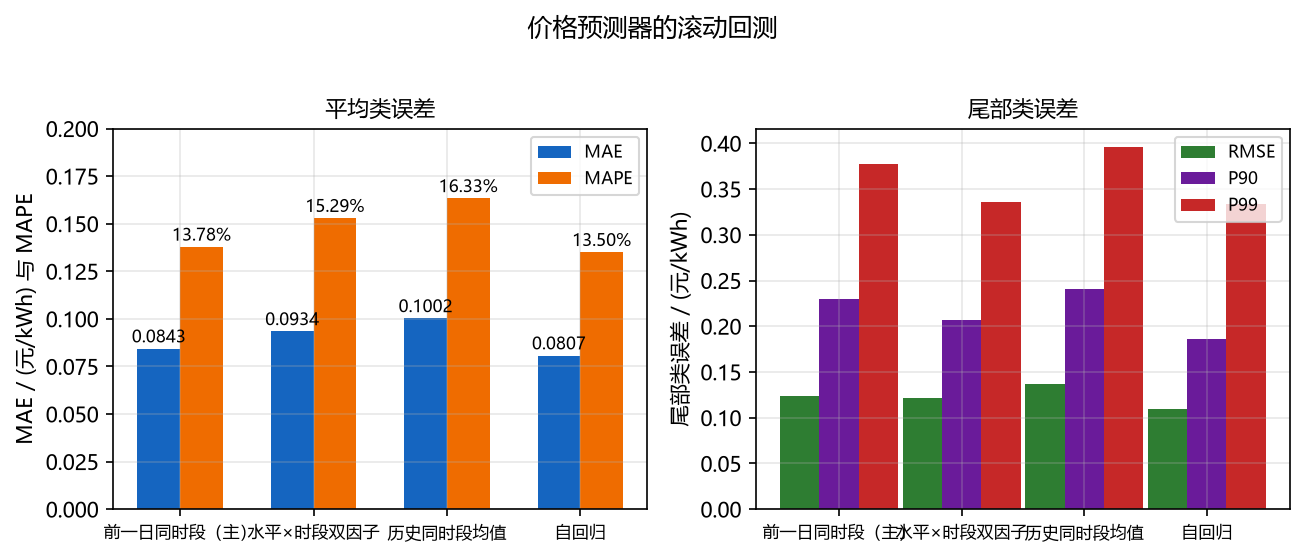
\includegraphics[width=0.80\textwidth]{fig15_p4_backtest.png}
\caption{价格预测器的滚动回测：平均类与尾部类指标的最优方向相反}
\label{fig:p4fc}
\end{figure}

\subsubsection{两条链的模型}

\textbf{链 \emph{4-2}（重算问题二）}。由于 0:00 不知道当天电价，链 \emph{4-2} 不能用“单一全年长时域线性规划”——那需要整年的价格序列。本文采用逐日向前递推：对每个交付日 $d$，用预测价与当天已知的实际负载、实际光伏求解一个单日规划

\begin{equation}
\min\ \sum_{i}\hat p^{(0)}_{d,i}b_{d,i}+\sum_{i}\alpha_{em}\hat p^{(0)}_{d,i}q^{em}_{d,i}
\quad\text{s.t.}\quad
b_i+q^{em}_i+PV^{act}_i\Delta t+q^{dis}_i=L_i\Delta t+c_i+s_i
\end{equation}

提交计划量后断言 $q\equiv b$，储电量按日边界连续性传递、终端自由。全年 365 次单日规划共约 11.9 s。

\textbf{链 \emph{4-3}（重算问题三）}。在问题三的三层结构上，把计划层的价格换成 $\hat p^{(0)}$（$\kappa_0\equiv1$）、调整层的价格换成式 (16) 的 $\hat p^{(m)}$，其余（预报降尺度、偏差分段、结算层闭式）与问题三相同。全年共 1460 个单日层，约 38.9 s。

\textbf{决策—结算分离与“价格预报误差的代价”}。同一组提交的决策量可以用两套价格分别计价：按决策层信念价计得 $C^{fc}$，按附件 4 实际价计得 $C^{act}$。本文以 $C^{act}$ 为唯一主结果，并把差额 $\Delta C^{price}=C^{act}-C^{fc}$ 定义为“价格预报误差的代价”单独报告。这一分解与问题三中“预报误差的代价”在结构上同构：一个是价格预测错了的代价，一个是光伏预测错了的代价。日前与实时市场的两结算与价格不确定性对储能收益的影响在文献中已被系统研究\cite{ref-krishnamurthy-2018-arbitrage-da-rt,ref-yang-2023-da-rt-shared-storage,ref-bottieau-2020-imbalance-settlement-forecast,ref-yang-2020-deviation-penalty-distribution,ref-paulauskas-2024-battery-scheduling-arbitrage}。

\subsubsection{主结果与三分项归因}

两条链的交付期主结果列于表~\ref{tab:p4main}。链 \emph{4-2} 的交付期费用为 $13\,006\,411.041148$ 元，链 \emph{4-3} 为 $15\,289\,050.714738$ 元，后者比前者高

\begin{equation}
2\,282\,639.673590=100\,230.446225+522\,512.788776+1\,659\,896.438588\quad(\text{单位：元})
\end{equation}

即差额可以\textbf{完全分解}为三项：计划口径差（两链计划层的价格与信息集不同导致的计划费用差异）、偏差结算制度（链 \emph{4-3} 独有的 $0.5\times/1.5\times$ 双向分段费用）与紧急购电（光伏预报误差在结算层形成的缺口），恒等式残差不超过 $10^{-6}$ 元（来自表格的六位小数舍入）。这一“三分项归因”是本文对问题四最主要的定量结论，它把一个 $2.28\times10^{6}$ 元的总差额变成了三条各自可解释、可单独核验的通道。

\begin{table}[htbp]
\centering
\small
\caption{问题四两条链的交付期主结果（334 天；费用单位：元，电量单位：kWh）}
\label{tab:p4main}
\begin{tabular}{p{5.4cm}rr}
\toprule
量 & 链 \emph{4-2} & 链 \emph{4-3} \\
\midrule
计划购电费 $C_{\text{plan}}^{act}$ & 13\,006\,411.041148 & 13\,106\,641.487373 \\
调整结算费 $C_{\text{adj}}^{act}$ & 0（无该项） & 522\,512.788776 \\
紧急购电费 $C_{\text{em}}^{act}$ & 0（机制性恒零） & 1\,659\,896.438588 \\
\textbf{总费用 $C_{\text{total}}^{act}$} & \textbf{13\,006\,411.041148} & \textbf{15\,289\,050.714738} \\
全期（365 天）总费用 & 14\,755\,884.322036 & 17\,181\,202.515506 \\
信念价口径费用 $C^{fc}$ & 12\,485\,620.202113 & 15\,030\,565.249034 \\
价格预报误差的代价 $\Delta C^{price}$ & 520\,790.839035 & 258\,485.465704 \\
计划购电量 $\sum b$ / 最终购电量 $\sum q$ & 20\,241\,516.374467 / 20\,241\,516.374467 & 20\,411\,764.664671 / 20\,807\,826.888962 \\
紧急购电量 $\sum q^{em}$ / 弃光量 $\sum s'$ & 0 / 990\,168.090312 & 394\,026.040750 / 1\,858\,369.774422 \\
净负荷（两链逐位相同） & 17\,939\,189.494967 & 17\,939\,189.494967 \\
\bottomrule
\end{tabular}
\end{table}

量级与上界自检：两链交付期费用均落在 $[3\times10^{6},5\times10^{7}]$ 元带内（日均分别为 38941.35 元与 45775.60 元）；用“完全不用储能”的可行策略构造的价格项上界为 17\,026\,782.858099 元与 18\,884\,193.220703 元，两链主值均低于上界，对应的储能价值为 4\,020\,371.82 元与 1\,737\,732.14 元。注意不能用附件 4 的最小电价构造下界——由于存在 0.0076 元/kWh 的极端低值，该下界不足实际费用的 1.2\%，不具判别力。

表~\ref{tab:p4a} 给出两条链在题面四个指定日期的结果。链 \emph{4-2} 报的是计划购电量 $b$、全天购电费等于计划费；链 \emph{4-3} 报的是最终购电量 $q$、全天购电费为三项之和。两链的数值必然不同（价格情景与决策结构均不同）：四个日期的紧急购电在链 \emph{4-2} 上全为零、在链 \emph{4-3} 上分别为 5、7、9、4 个合并区间。以 2025 年 3 月 20 日为例，链 \emph{4-2} 的六个 4 小时块充电量为 $[8082.85,3333.33,5658.77,5322.37,0.00,833.33]$ kWh、放电量为 $[0,6469.73,2777.38,254.72,6478.06,2836.94]$ kWh；链 \emph{4-3} 的充电量为 $[8082.85,3333.33,2856.65,6959.71,522.57,833.33]$ kWh、放电量为 $[0,6417.07,2313.92,250.65,6478.06,2836.94]$ kWh。两链该日的端部储电量均为 1200.0 kWh，属逐日滚动切片，与问题一的单日周期端点（恒 6000 kWh）语义不同。

\begin{table}[htbp]
\centering
\footnotesize
\caption{问题四：四个指定日期的指定时段购电量与全天合计（购电量单位：kWh，购电费单位：元）}
\label{tab:p4a}
\begin{tabular}{llrrrrrrrr}
\toprule
链 & 日期 & 10:00 & 12:00 & 14:00 & 16:00 & 18:00 & 20:00 & 全天购电量 & 全天购电费 \\
\midrule
\emph{4-2} & 2025-03-20 & 0.00 & 558.311667 & 0.00 & 507.324167 & 0.00 & 726.368333 & 66\,622.786007 & 41\,543.092634 \\
 & 2025-06-21 & 0.00 & 0.00 & 0.00 & 27.005000 & 0.00 & 0.00 & 32\,532.468316 & 15\,588.839124 \\
 & 2025-09-23 & 0.00 & 380.021250 & 0.00 & 493.582500 & 2.645000 & 61.911667 & 66\,265.421275 & 43\,331.557914 \\
 & 2025-12-21 & 0.00 & 906.683333 & 0.00 & 795.930417 & 712.633333 & 30.268333 & 94\,061.221951 & 70\,297.812713 \\
\emph{4-3} & 2025-03-20 & 0.00 & 553.563367 & 0.00 & 641.129717 & 0.00 & 726.368333 & 67\,656.452692 & 52\,443.510373 \\
 & 2025-06-21 & 0.00 & 0.00 & 0.00 & 112.922733 & 0.00 & 0.00 & 34\,007.160791 & 19\,429.156761 \\
 & 2025-09-23 & 0.00 & 358.668517 & 0.00 & 550.185183 & 2.645000 & 61.911667 & 68\,433.174459 & 50\,189.088074 \\
 & 2025-12-21 & 0.00 & 833.333333 & 0.00 & 806.735183 & 712.633333 & 30.268333 & 94\,508.735661 & 76\,068.603362 \\
\bottomrule
\end{tabular}
\end{table}

\subsubsection{机制解释}

\textbf{链 \emph{4-2} 的价格不确定性不产生能量缺口}（图~\ref{fig:p4a}）。决策层使用的信念价与结算层的实际价之间存在系统偏差，但链 \emph{4-2} 中负载与光伏在 0:00 即完全已知，价格预测错了只会让计划买贵或买便宜、不会造成供给不足，因此紧急购电恒为零（实测最大绝对值 $2.27\times10^{-13}$ kWh，属求解器容差级噪声，故表述为“机制性恒零”而非“逐位为零”）。价格误差的全部后果体现为 520\,790.839035 元的费用差。

\textbf{链 \emph{4-3} 的缺口来自光伏预报误差}。该链的紧急购电全部由“计划层与调整层用附件 3 预报、结算层用附件 2 实际”这一信息落差造成，与价格预测器无关：把 $\kappa_m$ 冻结为 1（即不做滚动校正）对实际费用几乎没有影响（相差 $1.49\times10^{-8}$ 元），但会显著改变信念价口径下的费用差（由 258\,485.47 元升至 573\,883.11 元）。这说明滚动价格校正的作用在于改善“决策者对账单的预期”，而非降低实际支出。

\textbf{两链的相对敏感性方向一致但幅度不同}。在 10 个共同情景上两链的费用变化方向同号；但在价格、负载与预测器三类扰动上，链 \emph{4-3} 反而比链 \emph{4-2} \emph{更不敏感}（分别低约 10\%、17\%、24\%），机制是调整层用当天已实现电价做了水平校正，形成部分对冲；相应地，链 \emph{4-3} 对光伏相关扰动远为敏感（为链 \emph{4-2} 的 42--65 倍）。这一“一边更钝、一边更锐”的对比正是三条归因通道的直接体现。

\begin{figure}[htbp]
\centering
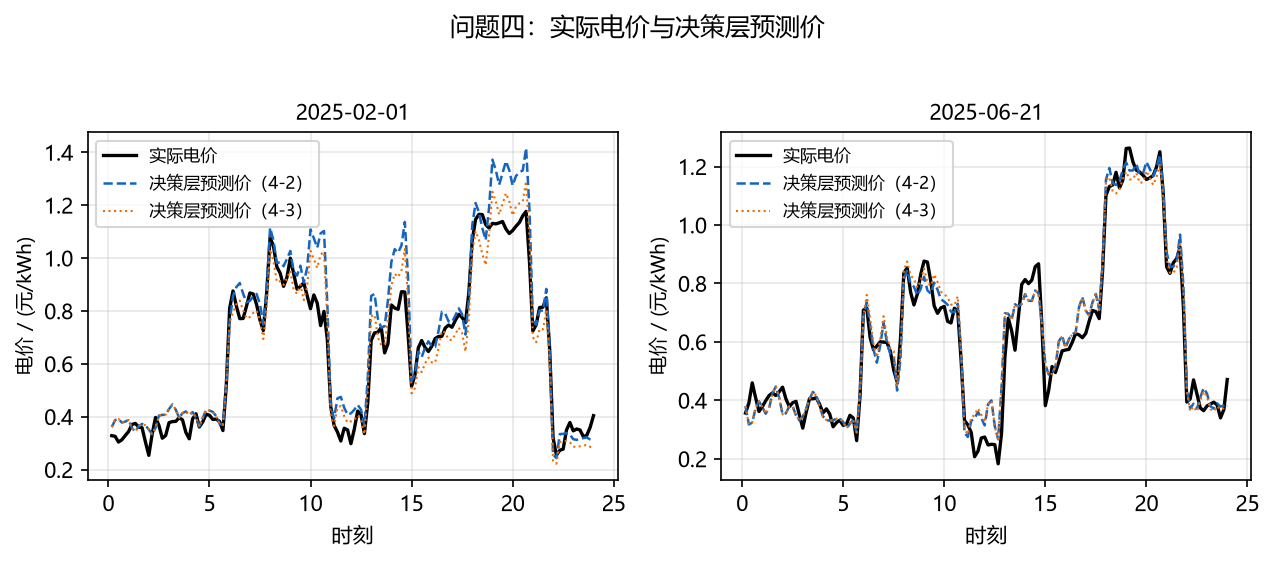
\includegraphics[width=0.80\textwidth]{fig14_p4_price.png}
\caption{决策层信念价与结算层实际价的分离（两链共用）}
\label{fig:p4a}
\end{figure}

\begin{figure}[htbp]
\centering
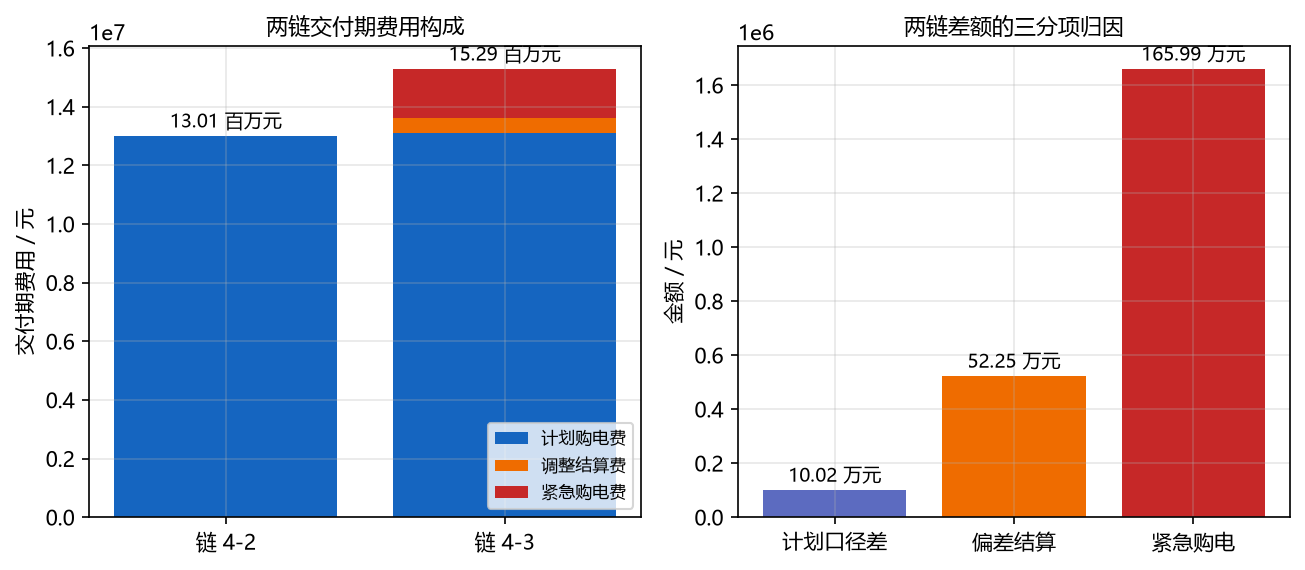
\includegraphics[width=0.80\textwidth]{fig16_p4_cost.png}
\caption{两链费用分项与交付期差额的三分项归因}
\label{fig:p4b}
\end{figure}

\subsubsection{稳健性与消融}

\textbf{鲁棒性}。链 \emph{4-2} 的 162 个情景全部成功、全部判据通过，分级为“稳定”；其最大敏感源是题面硬参数而非价格：往返效率的 $-20\%$ 档使费用上升 13.345\%，储电量上限收紧 20\% 使费用上升 5.141\%，而紧急购电倍数在六档上给出\textbf{完全相同}的费用（因紧急购电恒为零，该参数在本链上是空参数），初始储电量对交付期费用没有响应。链 \emph{4-3} 的 198 个情景中 195 个成功，3 个不可行情景全部是预注册的购电上限负对照（3500、4000、4500 kW）；另有 1 条判据未通过：光伏与负载的白噪声 $\sigma=10\%$ 族使费用均值上升 10.5919\%，超过 5\% 的预注册阈值，机制是紧急购电项的 $\max(0,\cdot)$ 凸性系统性抬高期望紧急购电，而所有受判样本均可行、恒等式残差为零，属结构性而非实现缺陷。据此链 \emph{4-3} 分级为“条件稳定（需给出适用边界）”：在 $\sigma\le5\%$ 的输入扰动下结论稳健，$\sigma=10\%$ 属超设计工况；结论\textbf{对价格侧稳健、对光伏侧不稳健}。本文不通过调参或放宽判据使该判据“通过”。

\textbf{消融与实现正确性锚点}。三组决定性对照（13 个对照项分链展开为 23 个算例）全部执行完毕。

第一，\textbf{退化情景复现（实现正确性锚点）}：把链 \emph{4-3} 的价格数据整体替换为附件 1 的单日曲线（逐日重复 365 次），其余输入与解的选择规则不变，此时“前一日同时段”预测在全年上精确成立、滚动校正因子恒为 1，模型理应退化为问题三。实测六项指标\textbf{逐位复现}问题三结果（全期 16\,179\,176.145228 元、交付期 14\,540\,616.335652 元、计划费 13\,885\,669.475555 元、调整费 563\,098.132533 元、紧急购电费 1\,730\,408.537141 元、交付期紧急购电量 391\,274.485914 kWh），六项相对差均不超过 $4.86\times10^{-13}$，远小于 $10^{-9}$ 的判据。这是本文对“问题四的实现是否正确”给出的最硬证据：一条完全独立于价格情景的退化路径必须精确回到已知答案。

第二，\textbf{两阶段随机规划对照（是否值得引入随机优化）}。为回答“点预测加确定性优化是否足够”，本文构造两阶段随机线性规划：第一阶段选择全天共用的计划购电量，第二阶段在每个价格情景内调整并结算；情景取自附件 4 的历史实际价格（对目标日取此前同型日的 144 点实际价向量、等概率，共 24 个情景），并裁剪为 12 个代表日的确定性等价大规划。结果显示，链 \emph{4-2} 上随机方案使同一窗口内的期望费用比点预测方案低 3.2860\%（13\,412.83 元），计划量的形状差异表现为“0--4 时与 16--20 时增购、4--8 时与 20--24 时减购”，即在低价时段多买、高价时段少买，属数量对冲。链 \emph{4-3} 上随机方案报告的降幅为 19.02\%，但这是因为预注册的追索结构使偏差变量恒为零、其期望费用与链 \emph{4-2} 逐位相同，因此\textbf{不得}把该降幅表述为“对冲在链 \emph{4-3} 上有 19\% 的收益”。综合判断：随机优化确实有收益，但在 12 个代表日窗口上不超过 3.3\%，且需要额外的场景建模与计算预算，本文据此维持“价格点预测 + 确定性线性规划”为主口径；这一判断也与“随机或鲁棒优化必须由问题结构与预算证明必要性”的方法论要求一致\cite{ref-akbari-2019-stochastic-robust-arbitrage,ref-oconnor-2025-conformal-price-forecast,ref-rawa-2023-mg-stochastic}。

第三，\textbf{滚动时域对照（前瞻深度）}。在决策时刻与承诺规则完全不变的前提下，只改变“优化时看多远”，把计划层的前瞻深度设为 $H\in\{1,3,7,14\}$ 天，窗口内的未来变量只用于优化、不进入承诺。$H=1$ 必须逐位复现主口径，实测全期与交付期费用差均为 0、整条储电量轨迹逐点差为 0，构成基线闸门。$H\ge3$ 时两链交付期费用分别再降 0.1785\% 与 0.1492\%，且前瞻深度在 $H=3$ 之后饱和（$H$ 由 3 增到 14 的费用增量仅 $-3.58$ 元与 $-5.49$ 元）。更重要的是，该对照直接回答了前文提出的结构性问题：主口径与 $H=1$ 下两链的日末储电量全部贴住下限 1200 kWh（364/365 与 365/365 天），而 $H\ge3$ 时日末储电量均值升至约 5335.9 与 5327.9 kWh、贴下限日数降至 30/365、唯一取值数增至 190 与 191。因此\textbf{“日边界不携带电量”只是“逐日 0:00 决策加终端自由”这一结构下的性质，不是与模型无关的普遍规律}，本文不作外推。此外如实登记一个反例：把两阶段随机与前瞻深度组合（24 个场景 $\times$ $H=3$、12 个代表日）后，期望费用反而比同窗点预测方案高 2.6959\%（11\,004.04 元），即“对冲加前瞻”在该窗口上\textbf{不叠加}收益；该结论只对窗口成立，本文不据此修改预注册设置。

最后，本文明确维持两条链的主口径不变：链 \emph{4-2} 为“前一日同时段预测价 + 逐日确定性线性规划”，链 \emph{4-3} 为“前一日同时段预测价 + 滚动水平校正 + 三层递推 + 双向分段结算”。模型族对照对费用结论的改变不超过 0.28\% 与 0.15\% 且无方向反转，退化情景锚点提供了实现正确性的硬证据，随机对照的收益幅度不足以证明更换主口径的必要性。


\section{模型的稳健性与灵敏度分析}

\subsection{实验设计原则}

四个问题的稳健性、灵敏度与消融分析遵循三条统一原则。第一，\textbf{检验标准事先设定}：核心结论、检验标准、阈值、扰动安排与样本量在计算前固定，事后不得修改；凡未能通过或被证伪的项一律如实列出，不通过调参、放宽阈值或挑选指标使其“通过”。第二，\textbf{不污染主方案}：随机规划、鲁棒优化、预测器替换、决策加密、前瞻深度等对照全部只进消融，主结果始终出自“确定性线性规划 + 题面规定的信息结构”。第三，\textbf{基线门槛}：每批扰动实验必须首先逐位复现主结果，否则整批作废，以保证对照之间的可比性——四问的基线复现相对差全部为 0（或不超过 $10^{-14}$）。

\subsection{稳定性分级汇总}

四问的扰动实验规模与结论汇总于表~\ref{tab:rob}。需要强调，分级所用的检验标准集合在计算前即已固定，因此“未通过”是结论而不是失败：它给出的是模型结论的适用边界。

\begin{table}[htbp]
\centering
\footnotesize
\caption{四个问题的扰动实验规模、分级与主要敏感源}
\label{tab:rob}
\begin{tabular}{p{1.5cm}rp{3.0cm}p{2.2cm}p{4.9cm}}
\toprule
问题 & 情景数 & 未通过检验标准 & 分级 & 主要敏感源与关键量 \\
\midrule
问题一 & 948（947 可行） & 无 & 稳定 & 往返效率 $\eta$（$0.9\to0.8$ 时 $+8.885\%$）；初值影响 $\le0.07\%$ \\
问题二 & 149 次全年 LP & 2 条（已归因） & 脆弱（需缩小适用范围） & $\eta$（$\pm10\%$ 使年度总量约 $\pm7\%$、单日量约 $\pm20\%$） \\
问题三 & 156 情景 & 1 条（噪声跨档均值） & 条件稳定（需给出适用边界） & $\eta$（单侧最大 10.9715\%）；初值对交付期无影响 \\
链 \emph{4-2} & 162 & 无 & 稳定 & 往返效率（$-20\%$ 档 $+13.345\%$）与储电量上限（$-20\%$ 档 $+5.141\%$） \\
链 \emph{4-3} & 198（195 成功） & 1 条（$\sigma=10\%$ 噪声族） & 条件稳定（需给出适用边界） & 光伏预报偏差（$+10\%$ 档 $+23.25\%$）与光伏噪声 \\
\bottomrule
\end{tabular}
\end{table}

\begin{figure}[htbp]
\centering
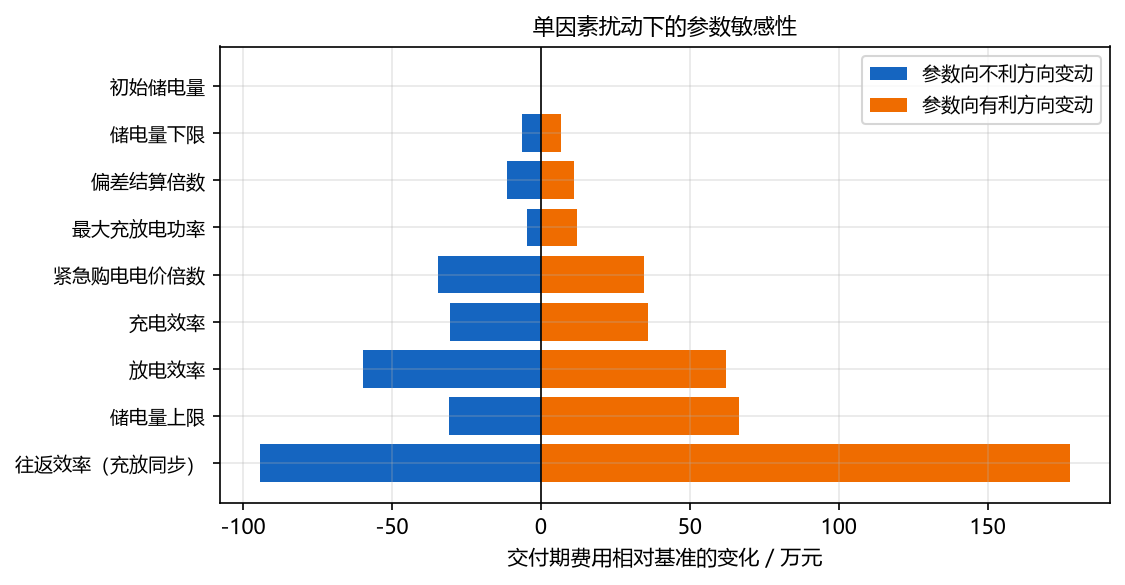
\includegraphics[width=0.490\textwidth]{fig19_robust_tornado.png}
\caption{参数敏感性的龙卷风图（问题三；其余问题为同类图）}
\label{fig:rob1}
\end{figure}

\subsection{敏感性主因的识别}

四个问题在敏感源上给出一致而清晰的图景，其中三点具有一般性。

第一，\textbf{往返效率是唯一一阶参数}。在四个问题上效率的影响都远大于其他参数：问题一 $\eta$ 由 0.9 降至 0.8 时费用上升 8.885\%、升至 1.0 时下降 7.828\%；问题二 $\eta$ 取 0.72 时费用上升 14.078\%，弹性约 $-0.66$ 至 $-0.70$；问题三单侧最大影响 10.9715\%；链 \emph{4-2} 为 13.345\%。相反，初始储电量的影响在所有问题上都可忽略（问题一不超过 0.07\%，问题二不超过 0.0042\%，问题三对交付期费用完全没有影响，链 \emph{4-2} 无响应）。这一对比有明确的物理解释：效率直接决定储能搬运电能的成本，而初值只影响开局的少量调节裕度；文献亦指出实际效率随荷电状态与功率变化，恒效率属工程简化，因此该参数既是最敏感项、也是最需要实测标定的一项\cite{ref-vykhodtsev-2022-bess-review,ref-huang-2022-dynamic-efficiency}。

第二，\textbf{敏感性的统计方式依赖必须随数字一起说明}。问题二的交付期费用稳定性检验之所以未通过，正是因为往返效率在日尺度量与年度总量上的敏感度相差约三倍（数值见问题二一节），因此本文在引用表~\ref{tab:p2a}、表~\ref{tab:p2b} 的单日数值时一律附带该声明。

第三，\textbf{“价格波动是第一不确定性源”按最大值统计时不成立}。这是本文如实列出的一个反例：按平均值统计时价格类扰动的影响确实居前，但按最大绝对值统计时价格类扰动的最大影响为 10.0\%，低于效率扰动的 13.345\%（链 \emph{4-2}）与 11.700\%（链 \emph{4-3}）。真正的一阶通道在链 \emph{4-2} 上是题面硬参数往返效率，在链 \emph{4-3} 上是光伏预报误差。本文不使用“价格是第一不确定性源”这一未经审慎表述的结论。

此外，链 \emph{4-3} 的未通过检验标准给出了本问题最有价值的适用边界：光伏与负载的白噪声在 $\sigma=5\%$ 下使费用上升约 3.9\%、在 $\sigma=10\%$ 下上升 11.2\%，而价格侧同类扰动影响明显更小。这说明在“预报驱动的三层决策 + 单侧紧急购电 + 非对称双向结算”这一结构下，\textbf{模型对光伏侧误差的暴露远大于对价格侧误差的暴露}，机制是紧急购电项的凸性把误差系统性地转化为费用。对工程实践的直接含义是：若要降低总费用，优先级应是提高光伏预报精度，而不是提高价格预报精度。

\subsection{模型族对比的整体结论}

跨四个问题的消融给出四条一致结论。

第一，\textbf{线性松弛无损，无需二元变量}。问题一中加入 144 个互补二元变量的整数模型与线性模型目标值完全相同；问题二中加入 52\,560 个二元变量的全规模整数模型只比线性模型高 4.355178 元（相对差 $3.2\times10^{-7}$），代价是求解时间从 5.8 s 增到 301.6 s 且未在时限内证明最优。引理 1 给出了这一现象的解析解释，也说明在规模较大时不必按混合整数规划建模。

第二，\textbf{独立第二实现与精确分解都逐位复现主结果}。问题二与问题三的独立第二实现以及问题二的精确逐日分解，都给出与主模型逐位相同的费用（做法与数值见问题二、问题三的模型族对照），这排除了主结果为实现假象的可能。

第三，\textbf{建模选择的影响可以大于机制价值}。问题三中把光伏预报的降尺度从整点锚定线性插值改为分段常数前向保持，会使费用上升 15.83\%（2\,561\,954.06 元），远大于调整机制本身 2.02\% 的价值；问题四中价格预测器的选择对费用影响不超过 0.28\%。这提示\textbf{数据处理方式的选择往往比模型结构的精细化更值得审慎对待}。

第四，\textbf{时域安排具有可量化的经济含义}。跨日状态连续、终端条件与日周期约束三项分别对应 26\,894.74 元、2217.08 元与 17\,135.02 元的费用差异；而“日边界不携带电量”这一在四条链上都出现的现象，被滚动时域对照证明只是“逐日决策加终端自由”结构的产物——把前瞻深度提高到 3 天以上，日末储电量即整体抬离下限（图~\ref{fig:rob2}，逐项数值见问题四的消融对照）。

\begin{figure}[htbp]
\centering
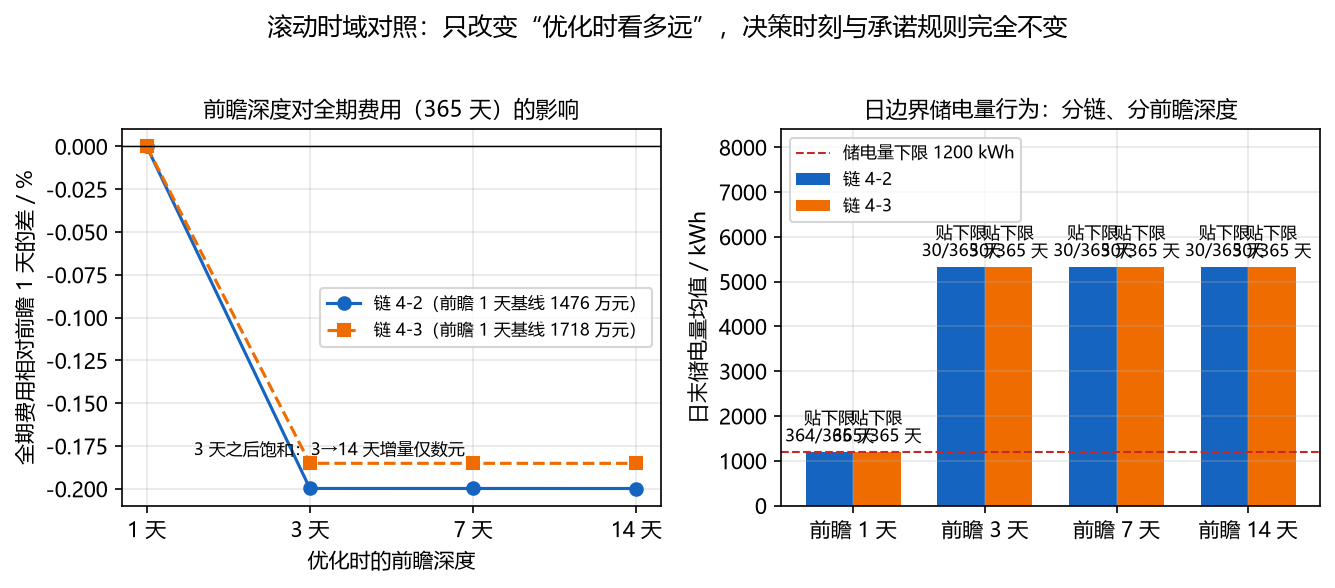
\includegraphics[width=0.535\textwidth]{fig20_rh_depth.png}
\caption{前瞻深度对费用的影响与日边界储电量行为：日边界不携带电量只在特定结构下成立}
\label{fig:rob2}
\end{figure}

\subsection{如实列出的反例与未通过项}

按“不得强凑单调性”的原则，本文记录以下六项与预期不符或未通过的结果：

\begin{enumerate}[leftmargin=2.2em,itemsep=1pt]
  \item 问题二的可行率检验未通过：唯一未通过的样本的目标值与基线逐位相同、解可行，未通过项是“返回解是否满足充放电互补性”，属退化最优面上的返回解选择问题。
  \item 问题二的交付表稳定检验未通过：$\eta=0.99$ 使 2025 年 6 月 21 日全天购电量下降 19.10\%，属有利方向的变化，但因检验标准取绝对值而被判失败；反向（$\eta=0.81$）最多使单日购电费上升 12.97\%。
  \item 问题三的噪声检验未通过：跨噪声幅度档的族间均值差 7.29\% 超过 3\% 阈值，而同幅度档内仅 0.06\%，属把两类统计量绑在同一检验标准里的设计问题。
  \item 链 \emph{4-3} 的噪声检验未通过：$\sigma=10\%$ 族均值上升 10.5919\% 超过 5\% 阈值，机制为紧急购电项的凸性，属结构性而非实现缺陷。
  \item 决策加密无收益：“每 3 小时”与“每 1 小时”的决策密度使费用分别上升 398.90 元与 590.07 元。本文不将其解读为“越密越差”，只记录“在题面给定的四个发布时刻下无收益”。
  \item 组合对照不叠加收益：两阶段随机与前瞻深度的组合方案在同一窗口内的期望费用比点预测方案高 2.6959\%（算例设定见问题四一节）。该结论只对 12 个代表日的窗口成立，本文不作外推。
\end{enumerate}

\subsection{对“是否需要更多预报、是否需要随机优化”的回答}

题面在问题三中提出了“是否需要引入其他时刻的预报制定调整购电策略”这一问题，本文把它拆成三个递进层面回答，并以计算成本作为约束；各层面的完整证据分别见问题三与问题四，此处给出汇总与取舍判断。

\textbf{层面一：要不要有调整？} 要。加入 6:00、12:00、18:00 三个调整时刻后的净收益为正（2.02\%），机制是减少 5 倍价紧急购电、代价是新增偏差违约金，两项金额已在问题三的费用分解中给出。

\textbf{层面二：在四个时刻之上是否还要加密？} 不需要。加密决策时刻并不增加信息量，只是把同一套预报用得更频繁，费用不降反升（金额见上一小节反例第 5 条）。

\textbf{层面三：要不要为了“看更远”而引入滚动优化？} 有收益但边际递减：两链交付期费用在 3 天前瞻上分别再降约 0.18\% 与 0.15\%，提高到 7 天与 14 天几乎不再改善。因此真正的价值来自“至少看 3 天”，而不是“看得越远越好”；同时该改动会使日末储电量脱离下限，从根本上改变模型的跨日行为。

\textbf{关于随机优化}：本文构造的两阶段随机规划对照在链 \emph{4-2} 上使同窗期望费用降低 3.2860\%，说明价格不确定性确实存在可对冲的部分；但链 \emph{4-3} 的随机对照因事先设定的自由追索而退化，其 19.02\% 的“降幅”不可作为对冲收益。综合收益幅度（不超过 3.3\%）、场景建模所需的历史样本量与额外计算预算，本文维持“价格点预测 + 确定性线性规划”为主方案，并明确指出：若要改换主方案，必须先补足价格与光伏误差的实测分布证据\cite{ref-akbari-2019-stochastic-robust-arbitrage,ref-oconnor-2025-conformal-price-forecast}。

\section{模型的评价与推广}

\subsection{模型的优点}

\textbf{第一，单一内核覆盖四个问题，口径可追溯。} 四个问题共用同一套 10 分钟粒度的线性规划内核，差异被完全参数化到时间、信息、结算与价格四个维度上（表~\ref{tab:param}）。变量定义、单位、参数值与时间范围在四问之间逐项一致，因此任何一个问题的实现都可以用同一套核验脚本检查，也使得“净负荷”“弃光量”这类与价格无关的量成为跨问题的硬校验点：四问的交付期净负荷均为 17\,939\,189.494967 kWh，问题二与链 \emph{4-2} 的弃光量均为 990\,168.090312 kWh，而费用必然不同——这既证明价格情景真实生效，也排除了“把上一问结果填到下一问”的可能。

\textbf{第二，实现正确性被当作一等目标，并且给出了硬证据。} 本文构造了三类相互独立的验证手段：一是\textbf{解析界}，为每个问题独立构造可行上界与下界（如问题一的“不用储能”策略给出 48052.046591 元），并明确指出因附件 4 存在 0.0076 元/kWh 的极端低值、以最小电价构造的下界不具判别力；二是\textbf{独立第二实现}，用不同的变量排序、变量消去与求解器设置重算，问题二中与主模型逐位相同；三是\textbf{退化情景锚点}，把链 \emph{4-3} 的价格换成附件 1 的单日曲线后必须逐位复现问题三的六个数值，实测相对差不超过 $4.86\times10^{-13}$（判据为 $10^{-9}$）。这三类手段把“实现是否正确”与“模型是否合适”两个问题彻底分开。

\textbf{第三，量纲与索引口径被显式固定，避免了最隐蔽的一类错误。} 本文明确规定：决策变量以 kWh 为单位、本身已含时间因子，费用表达式中不再乘 $\Delta t$；附件时间戳为所属时段的左端点，据此计划窗为 0:10 至 24:10。这两项约定看似细节，但一旦出错，费用会整体偏差 6 倍、全部时段整体错位，而结果“看起来仍然合理”。核验中对每一项都做了独立复算：若误乘 $\Delta t$，问题二交付期费用会落到约 $2.04\times10^{6}$ 元，与正确值相差 6 倍。

\textbf{第四，对“未通过”与“不利结果”的处理方式本身构成结论的一部分。} 四个问题共登记六项未通过判据与反例（表~\ref{tab:rob} 及相关正文），全部如实保留并逐条给出归因与适用边界。例如问题二的“脆弱”分级并非模型失败，而是准确指出了日尺度量对效率口径的高敏感性；链 \emph{4-3} 的“条件稳定”则准确指出了模型对光伏侧误差的暴露远大于价格侧——这一结论对实际运行有直接指导意义。

\textbf{第五，计算预算可控且不依赖特殊硬件。} 最大规模实例为问题二的 52\,560 个时段、315\,360 个变量、105\,120 条等式约束，在普通 CPU 上以稀疏矩阵求解约 5.8 s；问题三与链 \emph{4-3} 因分解为 1460 个单日层分别约需 42 s 与 39 s；全部鲁棒性与消融实验（合计上千次线性规划）在数十分钟内完成。这意味着模型可以被反复重算，适合作为决策支持工具\cite{ref-hai-2025-microgrid-price-ems}。

\subsection{模型的不足与适用边界}

\textbf{第一，确定性口径，预报误差的代价只能事后量化。} 主结果不含误差分布，也不含随机或鲁棒优化。问题三比问题二贵 2\,307\,565.50 元（$+18.863\%$），同净负荷下这一差额完全由预报误差造成；链 \emph{4-3} 比链 \emph{4-2} 贵 2\,282\,639.673590 元。本文用“价格预报误差的代价”（520\,790.839035 元与 258\,485.465704 元）与“光伏预报误差的代价”（紧急购电费 1\,659\,896.438588 元）分别量化了这两类误差，但都属事后度量；消融中的随机对照说明改进空间在 3\% 量级，不足以为更换主口径提供充分理由。

\textbf{第二，光伏降尺度不保块内能量。} 附件 3 只给整点预报，本文按整点锚定线性插值降到 10 分钟，块内平均功率为 $(2.5A_{k-1}+3.5A_k)/6$，一般不等于整点值。若改用分段常数前向保持，费用会上升 15.83\%，说明该项口径影响很大。本文的做法是保留双端整点信息并显式披露其能量性质，但这是本问题最需审慎的一项建模选择。

\textbf{第三，若干物理简化与题面参数的解释约定。} 模型假设常效率（不随荷电状态、功率与温度变化）、无自放电、购电无功率上限、无售电收益、不计储能折旧；其中“5000 kW 同时作用于并网点侧与电池侧、取更严者”是本文对题面参数的解释约定，不构成文献支持的结论。这些简化的影响方向已被量化：效率是唯一一阶敏感参数；若存在 3000 kW 的隐含购电上限，问题一的计划将不可行；在允许售电的情景下，松散的弃光上界会出现售出电量超过物理盈余的非物理套利。

\textbf{第四，文献证据等级不足。} 全文引用的文献均只达到摘要或元数据级，没有一条经过全文精读，因此引用只用于支撑框架级与机制级主张（“这类问题可以用线性规划建模”“分时电价下存在充放电套利动机”“偏差结算制度会影响储能策略”），不用于支撑任何公式级或定量级结论。题面给定的硬参数（紧急购电 5 倍价、偏差结算 0.5 倍与 1.5 倍）与本文的模型内推论（紧急购电恒零）同样不作为文献结论陈述。

\textbf{第五，最优面非唯一带来呈现上的技术限制。} 线性规划的最优调度面可能不唯一（储电量上下限两端均可能活跃），因此验收以约束残差、结构恒等式、目标值与交付表格为准，不比对逐点解的唯一性；本文统一采用字典序规则选取提交解，并量化了该规则的影响（问题三约 $10^{-4}$ 量级、链 \emph{4-3} 为 0.110739 元），说明它不改变任何结论，但读者不应把不同求解器返回的轨迹差异理解为模型不稳定。

\textbf{第六，前瞻深度与日边界行为的结构依赖。} 在“逐日 0:00 决策加终端自由”的组织方式下，四条链的日末储电量都贴住下限 1200 kWh。滚动时域对照证明这只是该结构的产物：把前瞻深度提高到 3 天以上，日末储电量均值即升至约 5330 kWh。因此本文不把“日边界不携带电量”写成普遍规律——这既是结论，也是对模型适用边界的提示。

\subsection{模型的改进方向}

其一，\textbf{提升证据等级}：取得关键文献全文，把引用从摘要级提升到全文级，重新核验公式级与定量级主张，尤其是偏差结算制度与价格预测方法相关的主张。

其二，\textbf{补充误差分布的实测证据}，在此基线上重新评估随机规划与分布鲁棒优化是否应作为主口径。本文已给出评估框架（两阶段随机、滚动时域、二者组合）与预注册判据，但结论依赖场景构造，需要价格与光伏误差的真实分布数据支撑。

其三，\textbf{细化储能物理模型}：引入与荷电状态、充放电功率相关的动态效率与自放电项，并在此基线上重估费用与稳定性分级；本文已量化效率的敏感性，可作为该改进价值的前置估计。

其四，\textbf{引入极短的实时平衡层}：题面允许在“其他时刻”获得预报，本文结论限于现有发布时刻下的决策频率；若能获得更频繁的预报发布，则需重新评估“信息供给增加”的价值。

\subsection{本文的创新点}

\textbf{创新点一：以“四个维度上的参数化”统一四个问题，并由此得到一个可复用的建模模板。} 本文没有为四个问题分别建模，而是先证明它们共享同一物理系统与同一数学结构，再把差异定位到时间、信息、结算、价格四个维度。这既减少了重复推导，更让“什么是这道题的难点”变得可判定：问题一、二在时域与终端口径，问题三在信息结构与降尺度，问题四在价格可观测性。

\textbf{创新点二：给出互补性引理，把“是否需要二元变量”从工程判断变成数学结论。} 通过对往返效率小于 1 的利用，本文证明同时充放电被严格支配，从而线性松弛无损；该结论被两个不同规模的整数模型对照独立验证（问题一中 144 个二元变量模型目标值完全相同，问题二中 52\,560 个二元变量模型仅差 $3.2\times10^{-7}$ 而耗时增加 50 倍）。这节省的不只是计算量，也避免了因引入大 M 常数而带来的数值脆弱性。

\textbf{创新点三：把“代价”做成可分解的量，而不是笼统的“不确定性影响”。} 本文对两类误差分别给出价格与金额，并在问题四中把两条链 2\,282\,639.673590 元的总差额完全分解为计划口径差、偏差结算与紧急购电三项（恒等式残差不超过 $10^{-6}$ 元）。这种分解使“哪一条通道更值得改进”有了定量答案：对链 \emph{4-3} 而言，降低光伏预报误差的收益远大于提高价格预测精度。

\textbf{创新点四：用“退化情景复现”构造实现正确性锚点。} 把链 \emph{4-3} 的价格换成附件 1 的单日曲线后，模型应当精确退化为问题三；实测六项指标逐位复现，相对差不超过 $4.86\times10^{-13}$。这一手法把“实现是否正确”变成一个可以客观判定的问题，且适用于任何“旧问题加新情景”的题目结构。

\textbf{创新点五：用滚动时域对照回答“结构性问题”，而非仅作灵敏度扫描。} “日边界储电量为什么总贴下限”无法通过参数扰动回答，因为它是结构性的。本文设计了对决策时刻与承诺规则完全不变、只改变“优化时看多远”的对照实验：前瞻深度为 1 天时逐位复现主口径，提高到 3 天以上时日末储电量均值升至约 5330 kWh、贴下限日数由 364/365 降至 30/365。这一“只改一个维度、其余严格不变”的设计使结论具有因果含义。

\textbf{创新点六：对不确定性与前瞻给出“三层递进回答”，把建议落到可执行的决策上。} 本文对“是否需要更多预报”给出层次分明的答案：需要调整机制、不需要加密决策时刻；需要一定前瞻（至少 3 天）、不需要无限前瞻；随机优化有收益（3.29\%）但幅度不足以替代主口径。同时指出优先级：由于模型对光伏侧误差的暴露远大于价格侧，提高光伏预报精度应是首要投入。


% ============ AI 工具使用声明（规范要求，置于参考文献前） ============
\section*{AI 工具使用声明}
本参赛队在竞赛过程中使用了 AI 工具，主要用于文献检索与元数据核验、模型与公式推导辅助、代码实现与调试、结果一致性检查与语言润色，详细使用情况见支撑材料。

% ============ 参考文献（GB/T 7714 数字标注） ============
% 参考文献（GB/T 7714；数字标注；按正文首次引用顺序排列）
\begin{thebibliography}{99}
\footnotesize
\setlength{\itemsep}{0.6pt}
\setlength{\parsep}{0pt}
\setlength{\parskip}{0pt}
\bibitem{ref-csee-2023-mg-ems-review}
(CSEE Journal of Power and Energy Systems，Crossref 未返回作者字段). Microgrid Energy Management with Energy Storage Systems: A Review[J]. CSEE Journal of Power and Energy Systems, 2023.
\bibitem{ref-moradi-2018-standalone}
Moradi Hadis, Esfahanian Mahdi, Abtahi Amir, Zilouchian Ali. Optimization and energy management of a standalone hybrid microgrid in the presence of battery storage system[J]. Energy, 2018.
\bibitem{ref-alguhi-2025-bess-operation}
Alguhi Ahmed A., Alotaibi Majed A. Optimal Operation of Battery Energy Storage Systems in Microgrid-Connected Distribution Networks for Economic Efficiency and Grid Security[J]. Energies, 2025.
\bibitem{ref-valibeygi-2020-battery-dispatch-soc}
Valibeygi Amir, de Callafon Raymond A. Optimal Battery Dispatch and Real-Time State of Charge Tracking for Microgrid Applications[C]. 2020 American Control Conference (ACC), 2020.
\bibitem{ref-wang-2024-complementarity}
Wang Qi, Wu Wenchuan, Lin Chenhui, Xu Shuwei, Wang Siyuan, Tian Jian. An exact relaxation method for complementarity constraints of energy storages in power grid optimization problems[J]. Applied Energy, 2024.
\bibitem{ref-nazir-2023-realizable-dispatch}
Nazir Nawaf, Almassalkhi Mads. Guaranteeing a Physically Realizable Battery Dispatch Without Charge-Discharge Complementarity Constraints[J]. IEEE Transactions on Smart Grid, 2023.
\bibitem{ref-grimaldi-2025-arbitrage-curtail}
Grimaldi Alberto, Minuto Francesco Demetrio, Perol Alessandro, Casagrande Silvia, Lanzini Andrea. Techno-economic optimization of utility-scale battery storage integration with a wind farm for wholesale energy arbitrage considering wind curtailment and battery degradation[J]. Journal of Energy Storage, 2025.
\bibitem{ref-qing-2025-pv-curtailment}
Qing Jiayuan, Jing Shi, Zhao Yincheng, Zhang Sen, Wan Hao, Cao Yihang. An Optimization for Capacity Configuration of Photovoltaic - Energy Storage Microgrid Considering the Solar Power Curtailment Rate[C]. 2025 7th Asia Energy and Electrical Engineering Symposium (AEEES), 2025.
\bibitem{ref-carpinelli-2013-dayahead-ilp}
Carpinelli G., Bracale A., Caramia P. The GREAT project: Integer linear programming-based day-ahead optimal scheduling of a DC microgrid[C]. 2013 12th International Conference on Environment and Electrical Engineering, 2013.
\bibitem{ref-alamir-2025-dayahead-multimg}
Alamir Nehmedo, Kamel Salah. Optimized Day-Ahead Scheduling of Cooperative Multi-Microgrid with Demand Response and Shapley Value-Based Cost Allocation[C]. 2025 26th International Middle East Power Systems Conference (MEPCON), 2025.
\bibitem{ref-lee-2020-purchase-cost-lp}
Lee Lae Yeop, Choi Seong Gon. Power Purchase Cost Minimization in Radial Microgrid Network with Linear Programming[C]. 2020 International Conference on Information and Communication Technology Convergence (ICTC), 2020.
\bibitem{ref-lin-2024-tou-industrial}
Lin Yangshu, Shao Yuhao, Yang Chao, Guo Wenxuan, Liu Weijie, Zheng Chenghang, Gao Xiang. Evaluation and optimization for integrated photo-voltaic and battery energy storage systems under time-of-use pricing in the industrial park[J]. Journal of Energy Storage, 2024.
\bibitem{ref-baloyi-2021-tou-arbitrage}
Baloyi T., Chowdhury S. Sizing and Selection of Battery Energy Storage System for Time of Use Arbitrage in a Commercial Building in South Africa[J]. 2021 IEEE PES/IAS PowerAfrica, 2021.
\bibitem{ref-olivieri-2020-residential-bess}
Olivieri Zachary T., McConky Katie. Optimization of residential battery energy storage system scheduling for cost and emissions reductions[J]. Energy and Buildings, 2020.
\bibitem{ref-shen-2026-peak-valley}
Shen Fangfei, Luo Quanming. A Multi-Objective Optimization Framework for Optimal Configuration of Battery Energy Storage System in Peak Shaving and Valley Filling Scenarios[J]. Applied Sciences, 2026.
\bibitem{ref-vykhodtsev-2022-bess-review}
Vykhodtsev Anton V., Jang Darren, Wang Qianpu, Rosehart William, Zareipour Hamidreza. A review of modelling approaches to characterize lithium-ion battery energy storage systems in techno-economic analyses of power systems[J]. Renewable and Sustainable Energy Reviews, 2022.
\bibitem{ref-huang-2022-dynamic-efficiency}
Huang Hongbo, Wang Hui, Cai Yang, Chen Xiwei, Li Tingting. Optimal Configuration of Fire-Storage Capacity Considering Dynamic Charge-Discharge Efficiency of Hybrid Energy Storage[J]. Frontiers in Energy Research, 2022.
\bibitem{ref-zhang-2015-dayahead-degradation}
Zhang Zhong, Wang Jianxue, Wang Xiuli. An improved charging/discharging strategy of lithium batteries considering depreciation cost in day-ahead microgrid scheduling[J]. Energy Conversion and Management, 2015.
\bibitem{ref-silvente-2015-rolling-horizon}
Silvente Javier, Kopanos Georgios M., Pistikopoulos Efstratios N., Espuña Antonio. A rolling horizon optimization framework for the simultaneous energy supply and demand planning in microgrids[J]. Applied Energy, 2015.
\bibitem{ref-holjevac-2017-receding-horizon}
Holjevac Ninoslav, Capuder Tomislav, Zhang Ning, Kuzle Igor, Kang Chongqing. Corrective receding horizon scheduling of flexible distributed multi-energy microgrids[J]. Applied Energy, 2017.
\bibitem{ref-hu-2020-mpc-overview}
Hu Jiefeng, Shan Yinghao, Guerrero Josep M., Ioinovici Adrian, Chan Ka Wing, Rodríguez José. Model predictive control of microgrids – An overview[J]. Renewable and Sustainable Energy Reviews, 2020.
\bibitem{ref-finnah-2021-da-intraday-adp}
Finnah Benedikt, Gönsch Jochen, Ziel Florian. Integrated day-ahead and intraday self-schedule bidding for energy storage systems using approximate dynamic programming[J]. European Journal of Operational Research, 2021.
\bibitem{ref-chazarra-2017-perfect-information}
Chazarra Manuel, Pérez-Díaz Juan I., García-González Javier. Value of perfect information of spot prices in the joint energy and reserve hourly scheduling of pumped storage plants[J]. Electric Power Systems Research, 2017.
\bibitem{ref-toubeau-2020-da-real-time}
Toubeau Jean-François, Bottieau Jérémie, De Grève Zacharie, Vallée François, Bruninx Kenneth. Data-Driven Scheduling of Energy Storage in Day-Ahead Energy and Reserve Markets With Probabilistic Guarantees on Real-Time Delivery[J]. IEEE Transactions on Power Systems, 2020.
\bibitem{ref-vanderveen-2016-balancing-market-design}
van der Veen Reinier A.C., Hakvoort Rudi A. The electricity balancing market: Exploring the design challenge[J]. Utilities Policy, 2016.
\bibitem{ref-herre-2020-imbalance-settlement}
Herre Lars. Impact of Imbalance Settlement System Design on Risk-Averse Energy Storage[C]. 2020 17th International Conference on the European Energy Market (EEM), 2020.
\bibitem{ref-joos-2018-integration-costs}
Joos Michael, Staffell Iain. Short-term integration costs of variable renewable energy: Wind curtailment and balancing in Britain and Germany[J]. Renewable and Sustainable Energy Reviews, 2018.
\bibitem{ref-almpantis-2024-minute-downscaling}
Diamantis Almpantis, Henrik Davidsson, Martin Andersson. A minute-resolution downscaling algorithm for high-resolution global irradiance time series[J]. Solar Energy Advances, 2024.
\bibitem{ref-barbieri-2017-very-short-term-pv}
Florian Barbieri, Sumedha Rajakaruna, Arindam Ghosh. Very short-term photovoltaic power forecasting with cloud modeling: A review[J]. Renewable and Sustainable Energy Reviews, 2017.
\bibitem{ref-stenzel-2016-temporal-resolution}
Peter Stenzel, Jochen Linssen, Johannes Fleer, Florian Busch. Impact of temporal resolution of supply and demand profiles on the design of photovoltaic battery systems for increased self-consumption[C]. 2016 IEEE International Energy Conference (ENERGYCON), 2016.
\bibitem{ref-li-2016-two-stage-rhc}
Zhongwen Li, Chuanzhi Zang, Peng Zeng, Haibin Yu. Combined Two-Stage Stochastic Programming and Receding Horizon Control Strategy for Microgrid Energy Management Considering Uncertainty[J]. Energies, 2016.
\bibitem{ref-bhattacharya-2018-multistage-storage}
Arnab Bhattacharya, Jeffrey P. Kharoufeh, Bo Zeng. Managing Energy Storage in Microgrids: A Multistage Stochastic Programming Approach[J]. IEEE Transactions on Smart Grid, 2018.
\bibitem{ref-elkazaz-2020-convex-mpc-rhc}
Mahmoud Elkazaz, Mark Sumner, David Thomas. Energy management system for hybrid PV-wind-battery microgrid using convex programming, model predictive and rolling horizon predictive control with experimental validation[J]. International Journal of Electrical Power \&amp; Energy Systems, 2020.
\bibitem{ref-danti-2019-intraday-rescheduling}
Irene Danti Lopez, Damian Flynn, Maël Desmartin, Marcelo Saguan. Intraday dispatch, energy storage and the value of re-scheduling in systems with high wind shares[C]. 2019 IEEE Power \&amp; Energy Society General Meeting (PESGM), 2019.
\bibitem{ref-matsumoto-2022-imbalance-design}
Takuji Matsumoto, Derek Bunn, Yuji Yamada. Mitigation of the Inefficiency in Imbalance Settlement Designs Using Day-Ahead Prices[J]. IEEE Transactions on Power Systems, 2022.
\bibitem{ref-asgarpoor-1995-deviation-penalty}
S. Asgarpoor, S.K. Panarelli. Expected Cost Penalty due to Deviation from Economic Dispatch for interconnected power systems[J]. IEEE Transactions on Power Systems, 1995.
\bibitem{ref-lago-2018-spot-price-deep-learning}
Jesus Lago, Fjo De Ridder, Bart De Schutter. Forecasting spot electricity prices: Deep learning approaches and empirical comparison of traditional algorithms[J]. Applied Energy, 2018.
\bibitem{ref-myttenaere-2016-mape-regression}
Arnaud de Myttenaere, Boris Golden, Bénédicte Le Grand, Fabrice Rossi. Mean Absolute Percentage Error for regression models[J]. Neurocomputing, 2016.
\bibitem{ref-chitsaz-2018-price-forecast-btm-storage}
Hamed Chitsaz, Payam Zamani-Dehkordi, Hamidreza Zareipour, Palak P. Parikh. Electricity Price Forecasting for Operational Scheduling of Behind-the-Meter Storage Systems[J]. IEEE Transactions on Smart Grid, 2018.
\bibitem{ref-khani-2015-online-adaptive-rtod}
Hadi Khani, Mohammad R. Dadash Zadeh. Online Adaptive Real-Time Optimal Dispatch of Privately Owned Energy Storage Systems Using Public-Domain Electricity Market Prices[J]. IEEE Transactions on Power Systems, 2015.
\bibitem{ref-staffell-2016-maximising-storage-value}
Iain Staffell, Mazda Rustomji. Maximising the value of electricity storage[J]. Journal of Energy Storage, 2016.
\bibitem{ref-mathaba-2014-price-forecast-benefit}
Tebello Mathaba, Xiaohua Xia, Jiangfeng Zhang. Analysing the economic benefit of electricity price forecast in industrial load scheduling[J]. Electric Power Systems Research, 2014.
\bibitem{ref-hodge-2018-forecast-value-storage}
Bri-Mathias Hodge, Carlo Brancucci Martinez-Anido, Qin Wang, Erol Chartan, Anthony Florita, Juha Kiviluoma. The combined value of wind and solar power forecasting improvements and electricity storage[J]. Applied Energy, 2018.
\bibitem{ref-krishnamurthy-2018-arbitrage-da-rt}
Dheepak Krishnamurthy, Canan Uckun, Zhi Zhou, Prakash R. Thimmapuram, Audun Botterud. Energy Storage Arbitrage Under Day-Ahead and Real-Time Price Uncertainty[J]. IEEE Transactions on Power Systems, 2018.
\bibitem{ref-yang-2023-da-rt-shared-storage}
Xiyun Yang, Liwei Fan, Xiangjun Li, Lingzhuochao Meng. Day-ahead and real-time market bidding and scheduling strategy for wind power participation based on shared energy storage[J]. Electric Power Systems Research, 2023.
\bibitem{ref-bottieau-2020-imbalance-settlement-forecast}
Jeremie Bottieau, Louis Hubert, Zacharie De Greve, Francois Vallee, Jean-Francois Toubeau. Very-Short-Term Probabilistic Forecasting for a Risk-Aware Participation in the Single Price Imbalance Settlement[J]. IEEE Transactions on Power Systems, 2020.
\bibitem{ref-yang-2020-deviation-penalty-distribution}
Jiajia Yang, Zhao Yang Dong, Fushuan Wen, Qixin Chen, Fengji Luo, Weijia Liu, Junpeng Zhan. A Penalty Scheme for Mitigating Uninstructed Deviation of Generation Outputs From Variable Renewables in a Distribution Market[J]. IEEE Transactions on Smart Grid, 2020.
\bibitem{ref-paulauskas-2024-battery-scheduling-arbitrage}
Nerijus Paulauskas, Vsevolod Kapustin. Battery Scheduling Optimization and Potential Revenue for Residential Storage Price Arbitrage[J]. Batteries, 2024.
\bibitem{ref-akbari-2019-stochastic-robust-arbitrage}
Alireza Akbari-Dibavar, Kazem Zare, Sayyad Nojavan. A hybrid stochastic-robust optimization approach for energy storage arbitrage in day-ahead and real-time markets[J]. Sustainable Cities and Society, 2019.
\bibitem{ref-oconnor-2025-conformal-price-forecast}
Ciaran O'Connor, Mohamed Bahloul, Roberto Rossi, Steven Prestwich, Andrea Visentin. Conformal Prediction for electricity price forecasting in the day-ahead and real-time balancing market[J]. Energy and AI, 2025.
\bibitem{ref-rawa-2023-mg-stochastic}
Rawa Muhyaddin, Al-Turki Yusuf, Sedraoui Khaled, Dadfar Sajjad, Khaki Mehrdad. Optimal operation and stochastic scheduling of renewable energy of a microgrid with optimal sizing of battery energy storage considering cost reduction[J]. Journal of Energy Storage, 2023.
\bibitem{ref-hai-2025-microgrid-price-ems}
Tao Hai, Narinderjit Singh Sawaran Singh, Farah Jamal. Energy management of a microgrid with integration of renewable energy sources considering energy storage systems with electricity price[J]. Journal of Energy Storage, 2025.
\end{thebibliography}


% ============ 附录（页数不限；规范第五条） ============
\section*{附录}
\addcontentsline{toc}{section}{附录}

\subsection*{附录 A\quad 支撑材料文件列表}

支撑材料包含五个结果文件、四个问题的完整可运行源程序，以及 AI 工具使用记录，清单如下。

\begin{center}
\small
\begin{tabular}{p{2.6cm}p{6.4cm}p{5.4cm}}
\toprule
类别 & 文件 & 说明 \\
\midrule
结果文件 & \texttt{result1.xlsx} & 问题一的计划购电量与储能充放电量 \\
结果文件 & \texttt{result2.xlsx} & 问题二的计划购电量、充放电量与紧急购电量 \\
结果文件 & \texttt{result3.xlsx} & 问题三的计划购电量、调整购电量、充放电量与紧急购电量 \\
结果文件 & \texttt{result4-2.xlsx} & 波动电价下重算问题二的完整结果 \\
结果文件 & \texttt{result4-3.xlsx} & 波动电价下重算问题三的完整结果 \\
源程序 & \texttt{prob01\_io.py}、\texttt{prob01\_model.py}、\texttt{run\_prob01.py} & 问题一：输入输出、模型构造、求解主程序 \\
源程序 & \texttt{prob02\_io.py}、\texttt{prob02\_model.py}、\texttt{run\_prob02.py} & 问题二：输入输出、模型构造、求解主程序 \\
源程序 & \texttt{prob03\_io.py}、\texttt{prob03\_model.py}、\texttt{run\_prob03.py} & 问题三：输入输出、三层模型、求解主程序 \\
源程序 & \texttt{prob04\_io.py}、\texttt{prob04\_model.py}、\texttt{prob04\_predict.py}、\texttt{run\_prob04.py} & 问题四：输入输出、两链模型、价格预测器、求解主程序 \\
其他 & 《AI 工具使用详情》 & AI 工具使用记录与人工复核说明 \\
\bottomrule
\end{tabular}
\end{center}

四个问题的求解程序共用同一套接口约定：输入为附件 \texttt{xlsx} 文件路径与结果模板路径，输出为解序列、交付表格、运行清单与交付工作簿。复现命令形如

\begin{center}
\small
\texttt{python run\_prob01.py --data 附件1.xlsx --template result1.xlsx --output <输出目录>}
\end{center}

所有程序均为 Python 3.14 编写，仅依赖 \texttt{numpy}、\texttt{scipy}、\texttt{openpyxl} 三个第三方库；线性规划统一调用 \texttt{scipy.optimize.linprog} 的 \texttt{highs} 方法在 CPU 上求解，不需要 GPU，也不依赖任何商业求解器。

\subsection*{附录 B\quad 求解程序清单}

\subsubsection*{B.1\quad 问题一：输入输出模块}

\lstinputlisting[language=Python]{../problems/microgrid_2025/prob01/versions/assumption_v003/code/prob01_io.py}

\subsubsection*{B.2\quad 问题一：模型构造模块}

\lstinputlisting[language=Python]{../problems/microgrid_2025/prob01/versions/assumption_v003/code/prob01_model.py}

\subsubsection*{B.3\quad 问题一：求解主程序}

\lstinputlisting[language=Python]{../problems/microgrid_2025/prob01/versions/assumption_v003/code/run_prob01.py}

\subsubsection*{B.4\quad 问题二：输入输出模块}

\lstinputlisting[language=Python]{../problems/microgrid_2025/prob02/versions/assumption_v001/code/prob02_io.py}

\subsubsection*{B.5\quad 问题二：模型构造模块}

\lstinputlisting[language=Python]{../problems/microgrid_2025/prob02/versions/assumption_v001/code/prob02_model.py}

\subsubsection*{B.6\quad 问题二：求解主程序}

\lstinputlisting[language=Python]{../problems/microgrid_2025/prob02/versions/assumption_v001/code/run_prob02.py}

\subsubsection*{B.7\quad 问题三：输入输出模块}

\lstinputlisting[language=Python]{../problems/microgrid_2025/prob03/versions/assumption_v001/code/prob03_io.py}

\subsubsection*{B.8\quad 问题三：三层模型模块}

\lstinputlisting[language=Python]{../problems/microgrid_2025/prob03/versions/assumption_v001/code/prob03_model.py}

\subsubsection*{B.9\quad 问题三：求解主程序}

\lstinputlisting[language=Python]{../problems/microgrid_2025/prob03/versions/assumption_v001/code/run_prob03.py}

\subsubsection*{B.10\quad 问题四：输入输出模块}

\lstinputlisting[language=Python]{../problems/microgrid_2025/prob04/versions/assumption_v001/code/prob04_io.py}

\subsubsection*{B.11\quad 问题四：两条链的模型模块}

\lstinputlisting[language=Python]{../problems/microgrid_2025/prob04/versions/assumption_v001/code/prob04_model.py}

\subsubsection*{B.12\quad 问题四：价格预测器}

\lstinputlisting[language=Python]{../problems/microgrid_2025/prob04/versions/assumption_v001/code/prob04_predict.py}

\subsubsection*{B.13\quad 问题四：求解主程序}

\lstinputlisting[language=Python]{../problems/microgrid_2025/prob04/versions/assumption_v001/code/run_prob04.py}


\end{document}
